% Preamble (mantido como na versão anterior, omitido por brevidade)
\documentclass[12pt]{article}
\usepackage[T1]{fontenc}
\usepackage[utf8]{inputenc}  
\usepackage{sbc-template}
\usepackage{pdflscape}
\usepackage{graphicx,url}
\usepackage[brazil]{babel}   
\usepackage{amsmath}
\usepackage{amsfonts}
\usepackage{amssymb}
\usepackage{changepage}
\usepackage{verbatim}
\usepackage{float}
\usepackage{cite}
\usepackage{graphicx}
\usepackage[ruled,vlined]{algorithm2e}
%\usepackage{amsmath} % Já carregado
\usepackage{adjustbox}
%\usepackage{float} % Já carregado
\usepackage{tabularx}
\graphicspath{ {images/} }
      
\sloppy
\title{Modelagem Preditiva de Visitas Médicas: Um Estudo Baseado em Múltiplos Classificadores}

\author{Tomás Nascimento Pimentel Barros\inst{1}, Tsang Ing Ren\inst{1}} 

\address{Centro de Informática -- Universidade Federal de Pernambuco (UFPE)\\
 Recife -- PE -- Brazil
 \email{tnpb@cin.ufpe.br, tir@cin.ufpe.br}
}

\begin{document} 

\maketitle
\setcounter{page}{1}

% Abstract (mantido como na versão anterior)
\begin{abstract}
O envelhecimento populacional no Brasil intensifica a demanda por serviços de saúde, tornando crucial a compreensão dos fatores que influenciam a frequência de visitas médicas por idosos. Este trabalho analisa dados da pesquisa \textit{National Poll on Healthy Aging} (NPHA) para modelar preditivamente a frequência de consultas médicas (0-1, 2-3, 4+ visitas) em indivíduos com 50 anos ou mais. Realizou-se uma análise exploratória e pré-processamento dos dados, seguida pela seleção de um subconjunto de 6 atributos relevantes (\textit{Physical Health, Dental Health, Employment, Prescription Sleep Medication, Race, Gender}). O desempenho de 13 algoritmos de classificação – incluindo modelos clássicos, técnicas de \textit{boosting} (XGBoost, LightGBM, CatBoost) e métodos de \textit{Dynamic Ensemble Selection} (DES), como KNORA-U, KNORA-E e META-DES – foi comparado utilizando validação cruzada estratificada (k=5) e otimização de hiperparâmetros com Optuna. Os resultados, avaliados pela métrica \textit{F1-Score} ponderado e testes estatísticos de Friedman e Nemenyi, indicaram diferenças significativas entre os modelos (p=0.003). \textit{Logistic Regression} obteve o melhor ranking médio (1.6), superando estatisticamente \textit{Naive Bayes} (11.2) e \textit{K-Nearest Neighbors} (9.8). Modelos DES e de \textit{boosting} apresentaram desempenho competitivo, embora sem diferença estatística significativa em relação ao melhor modelo nesta análise. O estudo contribui com \textit{insights} sobre preditores de visitas médicas e uma comparação metodológica robusta em um \textit{dataset} de relevância social e ainda pouco explorado.
\end{abstract}

% Seção 1: Introdução (mantida como na versão anterior)
\section{Introdução}
O cenário demográfico brasileiro atravessa uma transformação significativa, marcada pelo envelhecimento progressivo da população, com um aumento expressivo de indivíduos com 60 anos ou mais. Projeções indicam a continuidade desta tendência \cite{IBGE2019}, impondo desafios complexos a diversos setores sociais, com destaque para o sistema de saúde. O envelhecimento está associado a maior prevalência de condições crônicas e multimorbidades, elevando consideravelmente a demanda por serviços de saúde específicos para essa faixa etária \cite{MCKG2013}.

Diante da crescente pressão sobre os recursos sanitários, torna-se fundamental compreender os fatores que modulam a utilização desses serviços pela população idosa. Nesse contexto, Kim et al. \cite{KPSSP2014} investigaram a relação entre satisfação com a vida e frequência de visitas médicas em adultos acima de 50 anos, identificando uma associação inversa. Este achado sugere que maior frequência de consultas pode estar relacionada a menor satisfação com a vida, reforçando a necessidade de investigar os determinantes da utilização de serviços de saúde neste grupo populacional.

O impacto do envelhecimento no sistema de saúde brasileiro é amplamente reconhecido \cite{LidiaMota2022, mrejen2023envelhecimento}. O aumento da longevidade, embora um avanço social, implica maiores gastos, sobrecarga da infraestrutura e dos profissionais da área \cite{LidiaMota2022, mrejen2023envelhecimento}. Portanto, compreender os fatores que levam certos idosos a utilizarem os serviços de saúde com maior frequência é essencial para otimizar a alocação de recursos e garantir a sustentabilidade do sistema.

Este trabalho propõe-se a analisar um \textit{dataset} da pesquisa \textit{National Poll on Healthy Aging} (NPHA) \cite{NPHA2017}, focado em indivíduos com 50 anos ou mais, com dois objetivos principais. Primeiramente, realizar um estudo detalhado sobre este \textit{dataset}, incluindo análise exploratória e a primeira modelagem preditiva da frequência de visitas médicas nesta base. Dada a natureza dos dados, provenientes de uma pesquisa real com informações sobre saúde e bem-estar, espera-se que esta análise gere \textit{insights} valiosos. Uma modelagem precisa da variável-alvo (\textit{Number of Doctors Visited}) pode auxiliar na identificação de padrões de utilização, contribuindo para a otimização de recursos e fornecendo informações úteis para gestores de saúde.

Em segundo lugar, este trabalho visa comparar o desempenho de diferentes abordagens de classificação para esta tarefa. Avaliamos classificadores clássicos, algoritmos baseados em \textit{boosting} (XGBoost, LightGBM, CatBoost) e, com foco central, técnicas de \textit{Dynamic Ensemble Selection} (DES). O interesse particular nos métodos DES justifica-se por evidências de bom desempenho em problemas com \textit{datasets} de tamanho reduzido \cite{Cruz_2015}, como é o caso do NPHA \cite{ICPRAI2018SI}. Empregamos diversos algoritmos de \textit{machine learning}, incluindo \textit{Decision Trees}, \textit{Multinomial Logistic Regression}, \textit{Naive Bayes}, \textit{k-Nearest Neighbors} (k-NN), \textit{Support Vector Machines} (SVM), \textit{Neural Networks}, \textit{Random Forests}, \textit{Gradient Tree Boosting}, XGBoost, CatBoost, LightGBM e as técnicas DES específicas KNORA-U, KNORA-E e META-DES.

As seções subsequentes detalham a metodologia, apresentam os resultados, discutem suas implicações e concluem com as contribuições e direções futuras.

% Seção 2: Trabalhos Relacionados (mantida como na versão anterior)
\section{Trabalhos Relacionados}

Esta seção aborda os conceitos fundamentais de \textit{Multiple Classifier Systems} (MCS) e \textit{Dynamic Ensemble Selection} (DES), foco metodológico deste trabalho para a modelagem preditiva da frequência de visitas médicas em idosos.

\subsection{\textit{Dynamic Ensemble Classifiers}} 
Os \textit{Multiple Classifier Systems} (MCS) emergiram como uma abordagem robusta em \textit{machine learning}, visando aprimorar a capacidade de generalização em comparação ao uso de um único classificador \cite{Javed2024}. A premissa é que, ao combinar as predições de um \textit{ensemble} de classificadores diversos, os erros individuais podem ser compensados, resultando em uma decisão final mais precisa \cite{KO20081718}.

Um MCS é tipicamente construído em três fases: geração, seleção e integração \cite{Cruz_2015}. A geração cria um \textit{pool} de classificadores base, buscando diversidade através de técnicas como \textit{Bagging}, \textit{Boosting} ou \textit{Random Subspaces} \cite{KO20081718}. A integração combina as predições dos classificadores selecionados, usando regras como votação majoritária ou média de probabilidades \cite{Cruz_2015}.

A fase de seleção pode ser estática ou dinâmica \cite{Cruz_2015, KO20081718}. Na seleção estática, um subconjunto fixo é escolhido durante o treinamento para classificar todas as amostras futuras. Em contraste, a \textit{Dynamic Selection} (DS) opera de forma adaptativa: para cada nova amostra, um classificador ou \textit{ensemble} específico é selecionado \textit{on the fly} \cite{ICPRAI2018SI}.

A motivação para DS é que nenhum classificador individual é ótimo para todo o espaço de características; diferentes classificadores podem ser "especialistas" em subespaços distintos \cite{Cruz_2015, ICPRAI2018SI}. Técnicas DS buscam identificar os classificadores mais competentes para a amostra em questão, avaliando seu desempenho em uma "região de competência" local, definida ao redor da amostra de teste \cite{ICPRAI2018SI}. Esta região é comumente determinada usando os k-vizinhos mais próximos (\textit{k-NN}) da amostra de teste em um \textit{dataset} de validação, denominado \textit{Dynamic Selection Dataset} (DSEL) \cite{ICPRAI2018SI}.

As técnicas DS podem ser categorizadas em \textit{Dynamic Classifier Selection} (DCS), onde apenas o mais competente é selecionado, e \textit{Dynamic Ensemble Selection} (DES), onde um subconjunto dos mais competentes forma um \textit{ensemble} \cite{ICPRAI2018SI}. Abordagens DES são frequentemente preferidas por distribuírem o risco da estimativa de competência, resultando em maior robustez \cite{KO20081718}.

A adaptabilidade inerente das técnicas DES \cite{Javed2024} as torna promissoras para cenários complexos, como dados desbalanceados \cite{Wu2021, Javed2024}. Estudos indicam que DES pode superar métodos estáticos, especialmente com \textit{datasets} pequenos ou mal definidos \cite{Cruz_2015, ICPRAI2018SI}. A capacidade de ajustar a seleção com base na amostra permite explorar a especialização local dos membros do \textit{pool} de forma eficaz \cite{ICPRAI2018SI}.

\subsection{Aplicações de \textit{Dynamic Ensemble Classifiers} na Saúde} 
A área da saúde tem se beneficiado da aplicação de inteligência artificial (IA) e \textit{machine learning}, com métodos DES emergindo como ferramentas valiosas \cite{Javed2024}. A capacidade adaptativa dos DES é útil em cenários médicos com heterogeneidade de pacientes e complexidade clínica.

Aplicações proeminentes incluem o aprimoramento do diagnóstico médico via análise de imagens e dados patológicos, onde DES pode aumentar a precisão e auxiliar na detecção precoce de doenças \cite{Javed2024}. Na medicina personalizada, DES pode analisar dados complexos do paciente para prever respostas a tratamentos e otimizar planos terapêuticos \cite{Javed2024}.

A gestão de dados desbalanceados, comum em \textit{datasets} médicos, é outro campo onde DES se destaca. Wu et al. \cite{Wu2021} desenvolveram um modelo DES combinado com pré-processamento (\textit{SMOTE-ENN}) para detectar COVID-19 a partir de hemogramas, demonstrando sua eficácia em cenários com desbalanceamento de classes. Aplicações similares em avaliação de risco de crédito \cite{Wu2021} e estudos como o de Roy et al. \cite{ICPRAI2018SI} reforçam a vantagem de \textit{ensembles} dinâmicos para aprendizado multi-classe desbalanceado.

Adicionalmente, DES são aplicados no monitoramento remoto de pacientes, processando dados de sensores para prever problemas de saúde e permitir intervenções rápidas \cite{Javed2024}. Contudo, desafios persistem, incluindo a necessidade de dados de alta qualidade, complexidade computacional e considerações éticas sobre privacidade e interpretabilidade \cite{Javed2024}.

\subsection{Técnicas de \textit{Dynamic Selection}: KNORA e META-DES} 
As famílias KNORA (\textit{K-Nearest Oracles}) e META-DES destacam-se por suas abordagens distintas para estimar a competência dos classificadores base.

\subsubsection{KNORA (\textit{K-Nearest Oracles})}
Proposta por Ko et al. \cite{KO20081718}, KNORA avalia a competência de cada classificador base ($c_i$) do \textit{pool} ($C$) com base em seu desempenho na região de competência da amostra de teste ($x_q$), definida pelos $k$ vizinhos mais próximos no DSEL. As variantes principais são:

\begin{itemize}
    \item \textbf{KNORA-Eliminate (KNORA-E):} Seleciona $c_i$ para o \textit{ensemble} final ($C'$) somente se classificar corretamente \textit{todas} as $k$ amostras vizinhas. Se nenhum oráculo local perfeito é encontrado, $k$ é reduzido progressivamente. A decisão final é por votação majoritária em $C'$. Foca nos mais confiáveis localmente, mas pode gerar \textit{ensembles} pequenos ou vazios \cite{KO20081718}.

    \item \textbf{KNORA-Union (KNORA-U):} Seleciona $c_i$ se classificar corretamente \textit{pelo menos uma} das $k$ amostras vizinhas. Implementa votação ponderada, onde cada $c_i$ recebe votos iguais ao número de vizinhos que acertou. Tende a gerar \textit{ensembles} maiores, mas pode incluir classificadores menos robustos localmente \cite{KO20081718}.
\end{itemize}

Ambas as técnicas KNORA demonstraram eficácia, superando abordagens estáticas em certos cenários \cite{KO20081718}, e estão disponíveis na biblioteca DESlib.

\subsubsection{META-DES (\textit{Meta-Learning for Dynamic Ensemble Selection})} 
Desenvolvido por Cruz et al. \cite{Cruz_2015}, o \textit{framework} META-DES trata a seleção dinâmica como um problema de meta-aprendizado, treinando um "meta-classificador" ($\lambda$) para prever a competência de um classificador base $c_i$ para uma amostra $x_q$.

O processo envolve três fases:
\begin{enumerate}
    \item \textbf{Overproduction:} Geração de um \textit{pool} $C = \{c_1, ..., c_M\}$ usando o conjunto de treinamento $T$.
    
    \item \textbf{Meta-Training:} Para cada amostra $x_j$ no DSEL ($\mathcal{T}_{\lambda}$) e cada $c_i \in C$, extrai-se um vetor de meta-características ($v_{i,j}$) que codifica a competência de $c_i$ em relação a $x_j$ (e.g., acurácia local, consenso, confiança). O vetor $v_{i,j}$ é rotulado como "competente" ($\alpha_{i,j}=1$) se $c_i$ acertou $x_j$, ou "incompetente" ($\alpha_{i,j}=0$). O conjunto de meta-treinamento $\mathcal{T}_{\lambda}^*$ (com $N \times M$ vetores) é usado para treinar $\lambda$, beneficiando-se de um tamanho potencialmente maior que o DSEL original \cite{Cruz_2015}.
    
    \item \textbf{Generalization:} Para uma nova amostra $x_q$, extrai-se $v_{i,q}$ para cada $c_i$. O meta-classificador $\lambda$ prediz a probabilidade de competência. Classificadores acima de um limiar formam o \textit{ensemble} $C'$, e a decisão é por votação majoritária.
\end{enumerate}

A vantagem do META-DES é aprender a regra de seleção a partir dos dados, combinando múltiplas heurísticas \cite{Cruz_2015}. Experimentos indicam sua robustez, especialmente com dados limitados. Implementação disponível na DESlib.

% Seção 3: Metodologia (com legendas aprimoradas)
\section{Metodologia}

Esta seção descreve a metodologia empregada, baseada no \textit{framework CRISP-DM} \cite{crisp-dm}, abrangendo entendimento e pré-processamento do \textit{dataset}, análise exploratória, seleção de atributos, otimização de hiperparâmetros e avaliação dos modelos. O objetivo é extrair \textit{insights} sobre os fatores que influenciam a frequência de visitas médicas em idosos a partir das variáveis disponíveis.

\subsection{Visão Geral do \textit{Dataset}} 

% Tabela 1 - Legenda Aprimorada
\begin{table}[htbp]
\centering
\caption{Metadados do \textit{Dataset} NPHA: Nome, Contagem de Valores Não Nulos e Tipo de Dado para Cada Atributo Original} % Legenda Aprimorada
\label{tab:dados} 
\resizebox{\textwidth}{!}{
\begin{tabular}{|c|l|c|c|}
\hline
\# & \multicolumn{1}{c|}{\textbf{Coluna}} & \textbf{Contagem Não-Nula} & \textbf{Tipo de Dado} \\ 
\hline
1 & \textit{Age} & 714 não-nulos & int64 \\
2 & \textit{Physical\_Health} & 714 não-nulos & int64 \\
3 & \textit{Mental\_Health} & 714 não-nulos & int64 \\
4 & \textit{Dental\_Health} & 714 não-nulos & int64 \\
5 & \textit{Employment} & 714 não-nulos & int64 \\
6 & \textit{Stress\_Keeps\_Patient\_from\_Sleeping} & 714 não-nulos & int64 \\
7 & \textit{Medication\_Keeps\_Patient\_from\_Sleeping} & 714 não-nulos & int64 \\
8 & \textit{Pain\_Keeps\_Patient\_from\_Sleeping} & 714 não-nulos & int64 \\
9 & \textit{Bathroom\_Needs\_Keeps\_Patient\_from\_Sleeping} & 714 não-nulos & int64 \\
10 & \textit{Unkown\_Keeps\_Patient\_from\_Sleeping} & 714 não-nulos & int64 \\ 
11 & \textit{Trouble\_Sleeping} & 714 não-nulos & int64 \\
12 & \textit{Prescription\_Sleep\_Medication} & 714 não-nulos & int64 \\
13 & \textit{Race} & 714 não-nulos & int64 \\
14 & \textit{Gender} & 714 não-nulos & int64 \\
15 & \textit{Number\_of\_Doctors\_Visited} & 714 não nulos & int64 \\
\hline
\end{tabular}
}
\end{table}


Utilizamos dados do \textit{National Poll on Healthy Aging} (NPHA) \cite{NPHA2017}, pesquisa com adultos $\ge$ 50 anos sobre saúde e assistência médica. O \textit{dataset} foi selecionado por suas variáveis relevantes (saúde mental, dentária, sono, medicação) e pela oportunidade de gerar \textit{insights} inéditos através de modelagem.

A base original continha 714 instâncias e 14 atributos inteiros, sem dados ausentes (Tabela~\ref{tab:dados}). A variável-alvo, \textit{Number\_of\_Doctors\_Visited}, também é inteira. As variáveis são predominantemente ordinais ou binárias (Tabela~\ref{tab:variaveis_pacientes}).

% Tabela 2 - Legenda Aprimorada
\begin{table}[htbp]
\centering
\caption{Descrição Detalhada dos Atributos do \textit{Dataset} NPHA: Semântica e Esquema de Codificação Original} % Legenda Aprimorada
\label{tab:variaveis_pacientes} 
\resizebox{\textwidth}{!}{
\begin{tabular}{|p{6cm}|p{8cm}|p{8cm}|}
\hline
\textbf{Feature} & \textbf{Descrição} & \textbf{Rótulo / Codificação} \\ 
\hline
\textit{Number of Doctors Visited} & Número total de médicos distintos visitados & 1: 0-1; 2: 2-3; 3: 4+ \\ 
\hline
\textit{Age} & Grupo etário do paciente & 1: 50-64, 2: 65-80 \\
\hline
\textit{Physical Health} & Autoavaliação do bem-estar físico & 0: Recusado, 1: Ruim, 2: Regular, 3: Bom, 4: Muito Bom, 5: Excelente \\
\hline
\textit{Mental Health} & Autoavaliação da saúde mental/psicológica & 0: Recusado, 1: Ruim, 2: Regular, 3: Bom, 4: Muito Bom, 5: Excelente \\
\hline
\textit{Dental Health} & Autoavaliação da saúde bucal/dental & 0: Recusado, 1: Ruim, 2: Regular, 3: Bom, 4: Muito Bom, 5: Excelente \\
\hline
\textit{Employment} & Situação de emprego/trabalho & 0: Não trab./Recusado, 1: Aposentado, 2: Tempo parcial, 3: Tempo integral \\ 
\hline
\textit{Stress Keeps Patient from Sleeping} & Estresse afeta o sono & 0: Não, 1: Sim \\ 
\hline
\textit{Medication Keeps Patient from Sleeping} & Medicação afeta o sono & 0: Não, 1: Sim \\ 
\hline
\textit{Pain Keeps Patient from Sleeping} & Dor física perturba o sono & 0: Não, 1: Sim \\ 
\hline
\textit{Bathroom Needs Keeps Patient from Sleeping} & Necessidade de ir ao banheiro afeta o sono & 0: Não, 1: Sim \\ 
\hline
\textit{Unknown Keeps Patient from Sleeping} & Fatores não identificados afetam o sono & 0: Não, 1: Sim \\ 
\hline
\textit{Trouble Sleeping} & Dificuldades gerais com o sono & 0: Não, 1: Sim \\ 
\hline
\textit{Prescription Sleep Medication} & Uso de medicação prescrita para dormir & 0: Recusado, 1: Não usa, 2: Usa ocasional., 3: Usa regular. \\ 
\hline
\textit{Race} & Origem racial/étnica & -2: N/A, -1: Recusado, 1: Branco N-Hisp, 2: Negro N-Hisp, 3: Outro N-Hisp, 4: Hispânico, 5: 2+ Raças N-Hisp \\ 
\hline
\textit{Gender} & Identidade de gênero & -2: N/A, -1: Recusado, 1: Masculino, 2: Feminino \\ 
\hline
\end{tabular}
}
\end{table}

\subsection{Análise Exploratória dos Dados} 

Realizamos uma análise exploratória detalhada (AED) para identificar padrões, distribuições e relações entre variáveis, orientando a modelagem subsequente e fornecendo \textit{insights} preliminares sobre os fatores associados à frequência de visitas médicas.

% Figura 1 - Legenda Aprimorada
\begin{figure}[htbp]
    \centering
    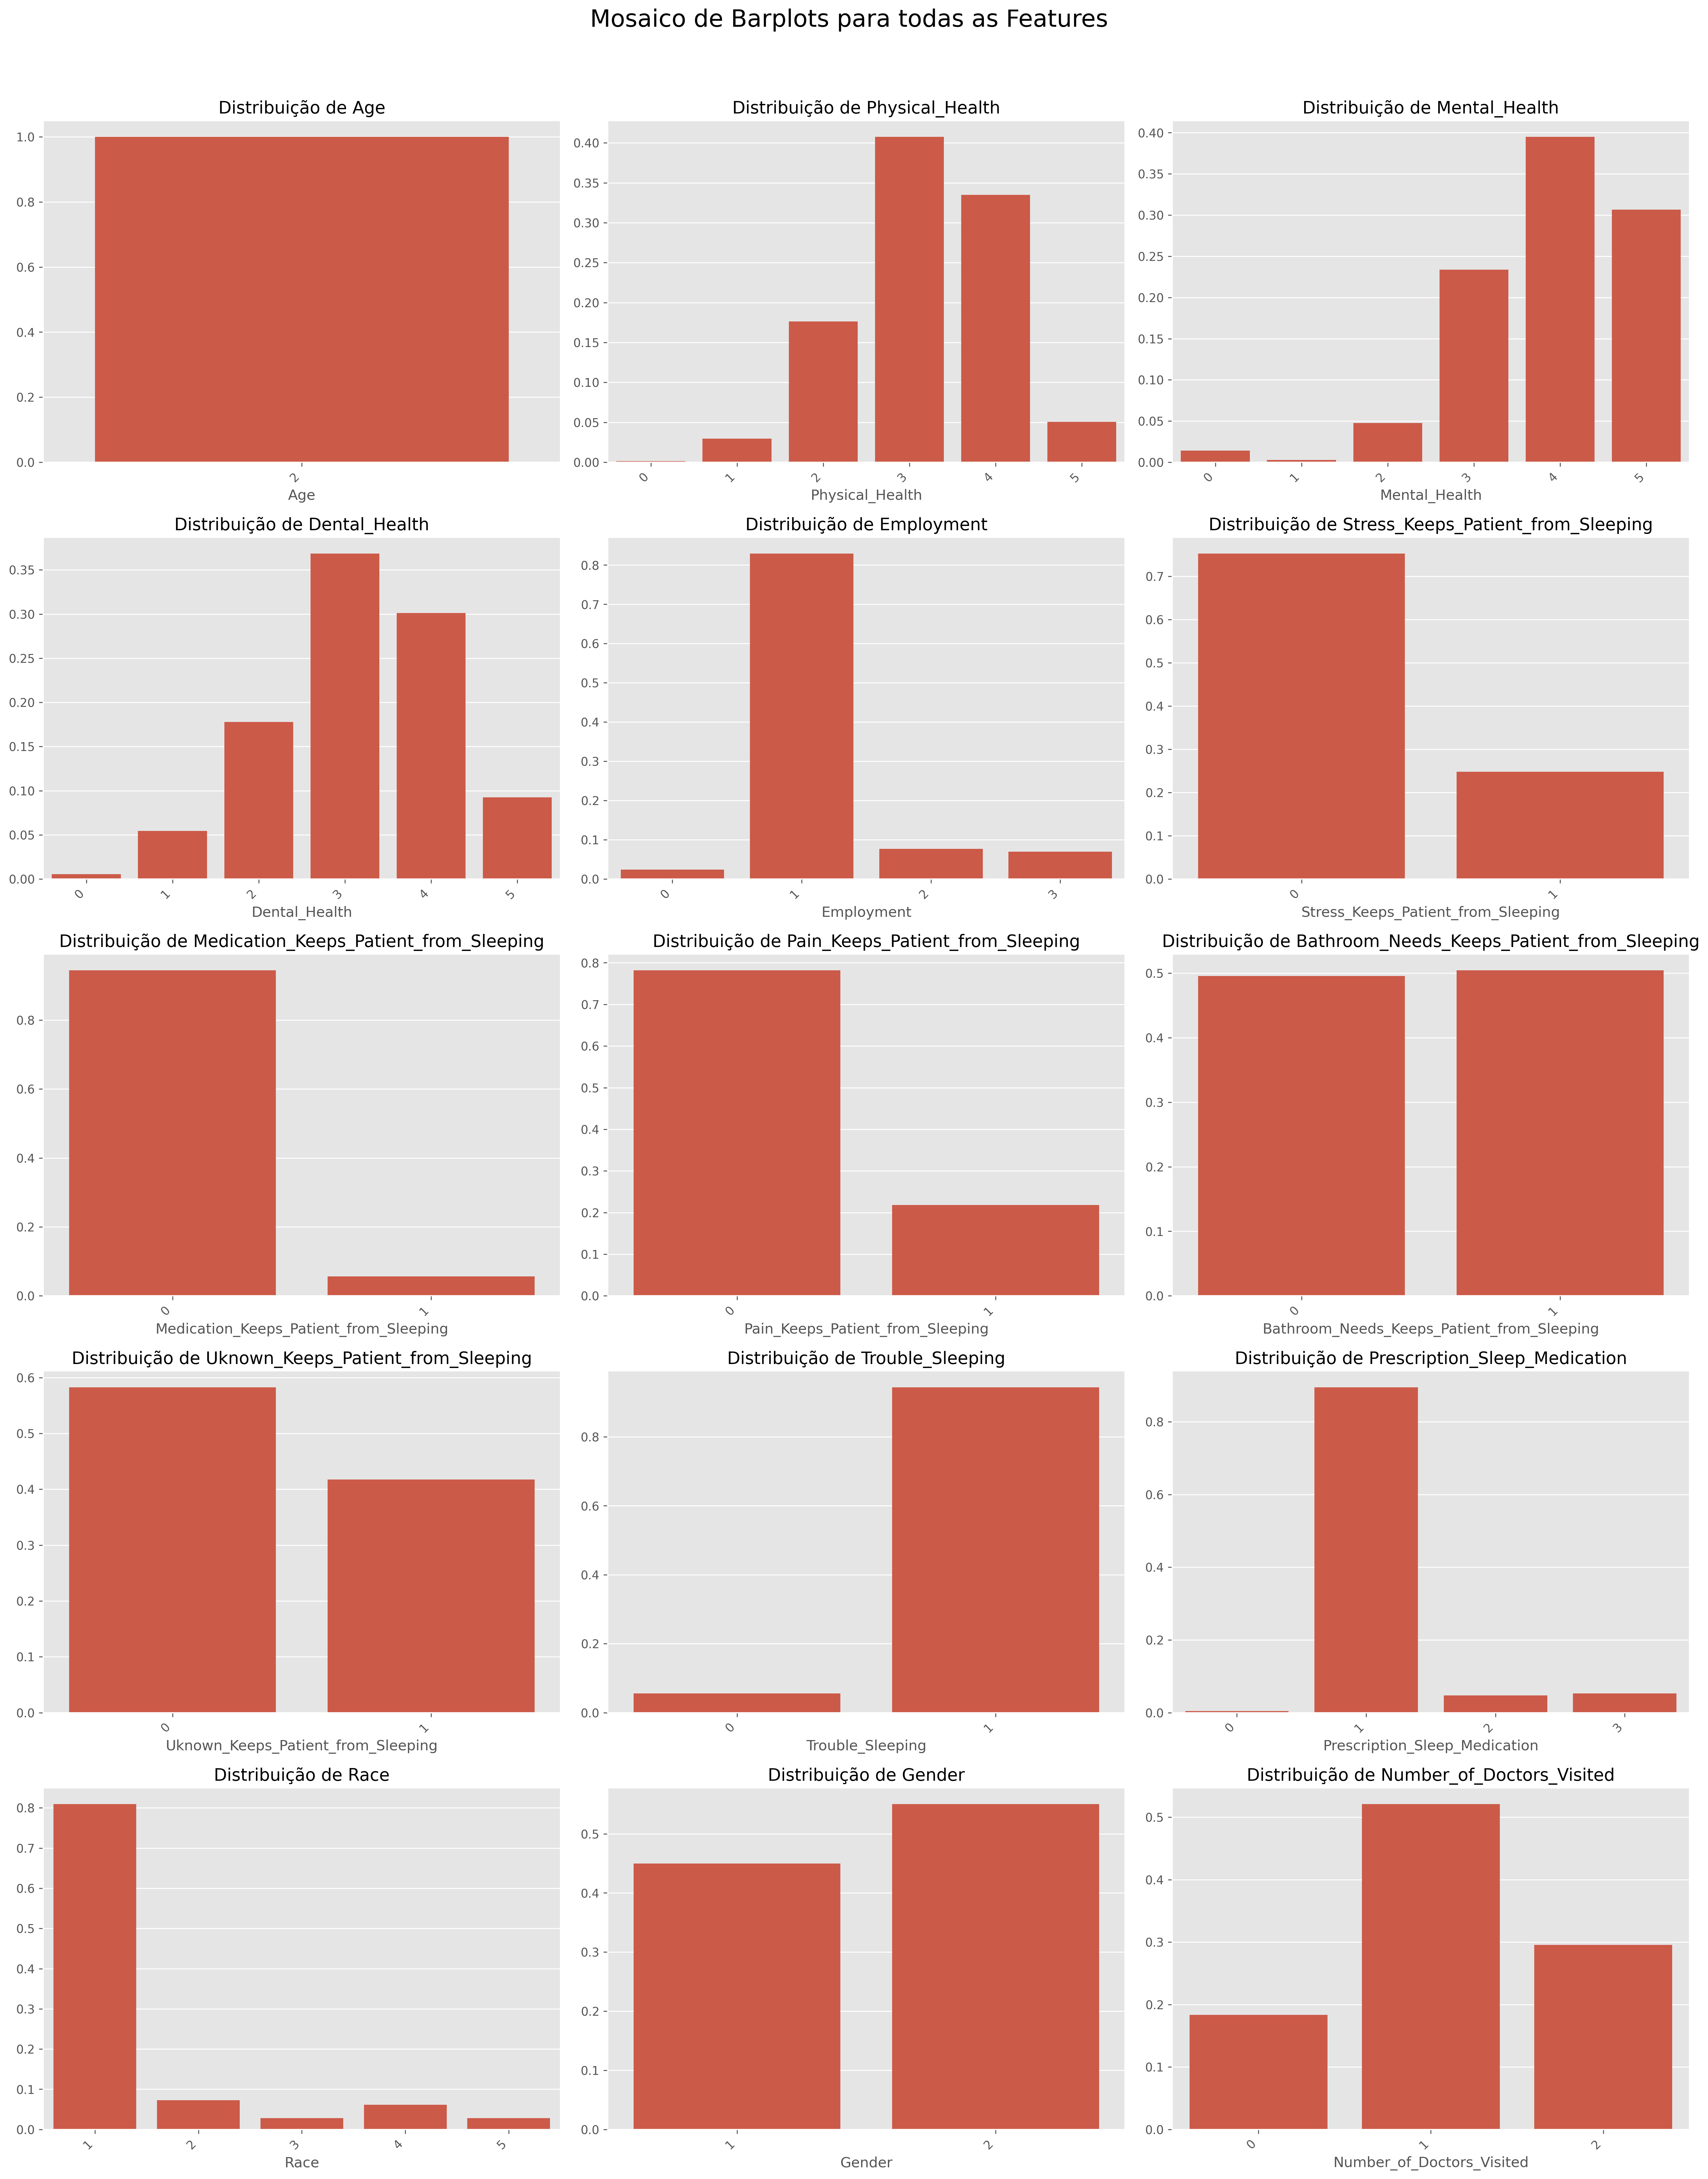
\includegraphics[width=\textwidth]{images/data_barplot_mosaic.png}
    \caption{Análise da Distribuição Univariada: Mosaico de Gráficos de Barras para Cada Atributo do \textit{Dataset} NPHA Original} % Legenda Aprimorada
    \label{fig:mosaico_dados_barplot}
\end{figure}

\subsubsection{Análise da Distribuição das Variáveis}

A Figura~\ref{fig:mosaico_dados_barplot} apresenta a distribuição de cada variável:
\begin{itemize}
    \item \textit{Age}: Homogênea (valor 2: 65-80 anos), limitando seu poder preditivo.
    \item \textit{Physical Health}: Concentração (59\%) em "boa" a "excelente" (valores 3-5), consistente com dados do HHS \cite{ACL_AoA2018}.
    \item \textit{Mental Health}: Alta concentração (98\%) em "razoável" a "excelente" (valores 2-5), alinhada com dados do SAMHSA \cite{SAMHSA2017}.
    \item \textit{Dental Health}: Predominância (59\%) de "boa" ou "muito boa" (valores 3-4).
    \item \textit{Employment}: Maioria aposentada (83\%, valor 1).
    \item \textit{Stress Keeps Patient from Sleeping}: 75\% não relatam problemas de sono por estresse (valor 0).
    \item \textit{Medication Keeps Patient from Sleeping}: Apenas 10\% relatam problemas de sono por medicação (valor 1).
    \item \textit{Pain Keeps Patient from Sleeping}: 80\% não relatam problemas de sono por dor (valor 0).
    \item \textit{Bathroom Needs Keeps Patient from Sleeping}: Distribuição equilibrada (~50\% afetados, valor 1).
    \item \textit{Unknown Keeps Patient from Sleeping}: Parcela significativa (40\%) relata dificuldades por causas não identificadas (valor 1).
    \item \textit{Trouble Sleeping}: Alta prevalência de problemas de sono (~90\%, valor 1).
    \item \textit{Prescription Sleep Medication}: Maioria (~90\%) não utiliza medicação prescrita para dormir.
    \item \textit{Race}: Concentração em "Brancos, Não-Hispânicos" (~80\%, valor 1).
    \item \textit{Gender}: Relativamente equilibrada (55\% feminino, valor 2).
    \item \textit{Number of Doctors Visited} (Variável-Alvo): Desbalanceada, com predominância da classe intermediária (2-3 médicos, ~50\%, valor 1), seguida por 4+ médicos (~30\%, valor 2) e 0-1 médicos (~20\%, valor 0).
\end{itemize}

\subsection{Análise de Correlações Bivariadas} 

% Figura 2 - Legenda Aprimorada
\begin{figure}[htbp]
    \centering
    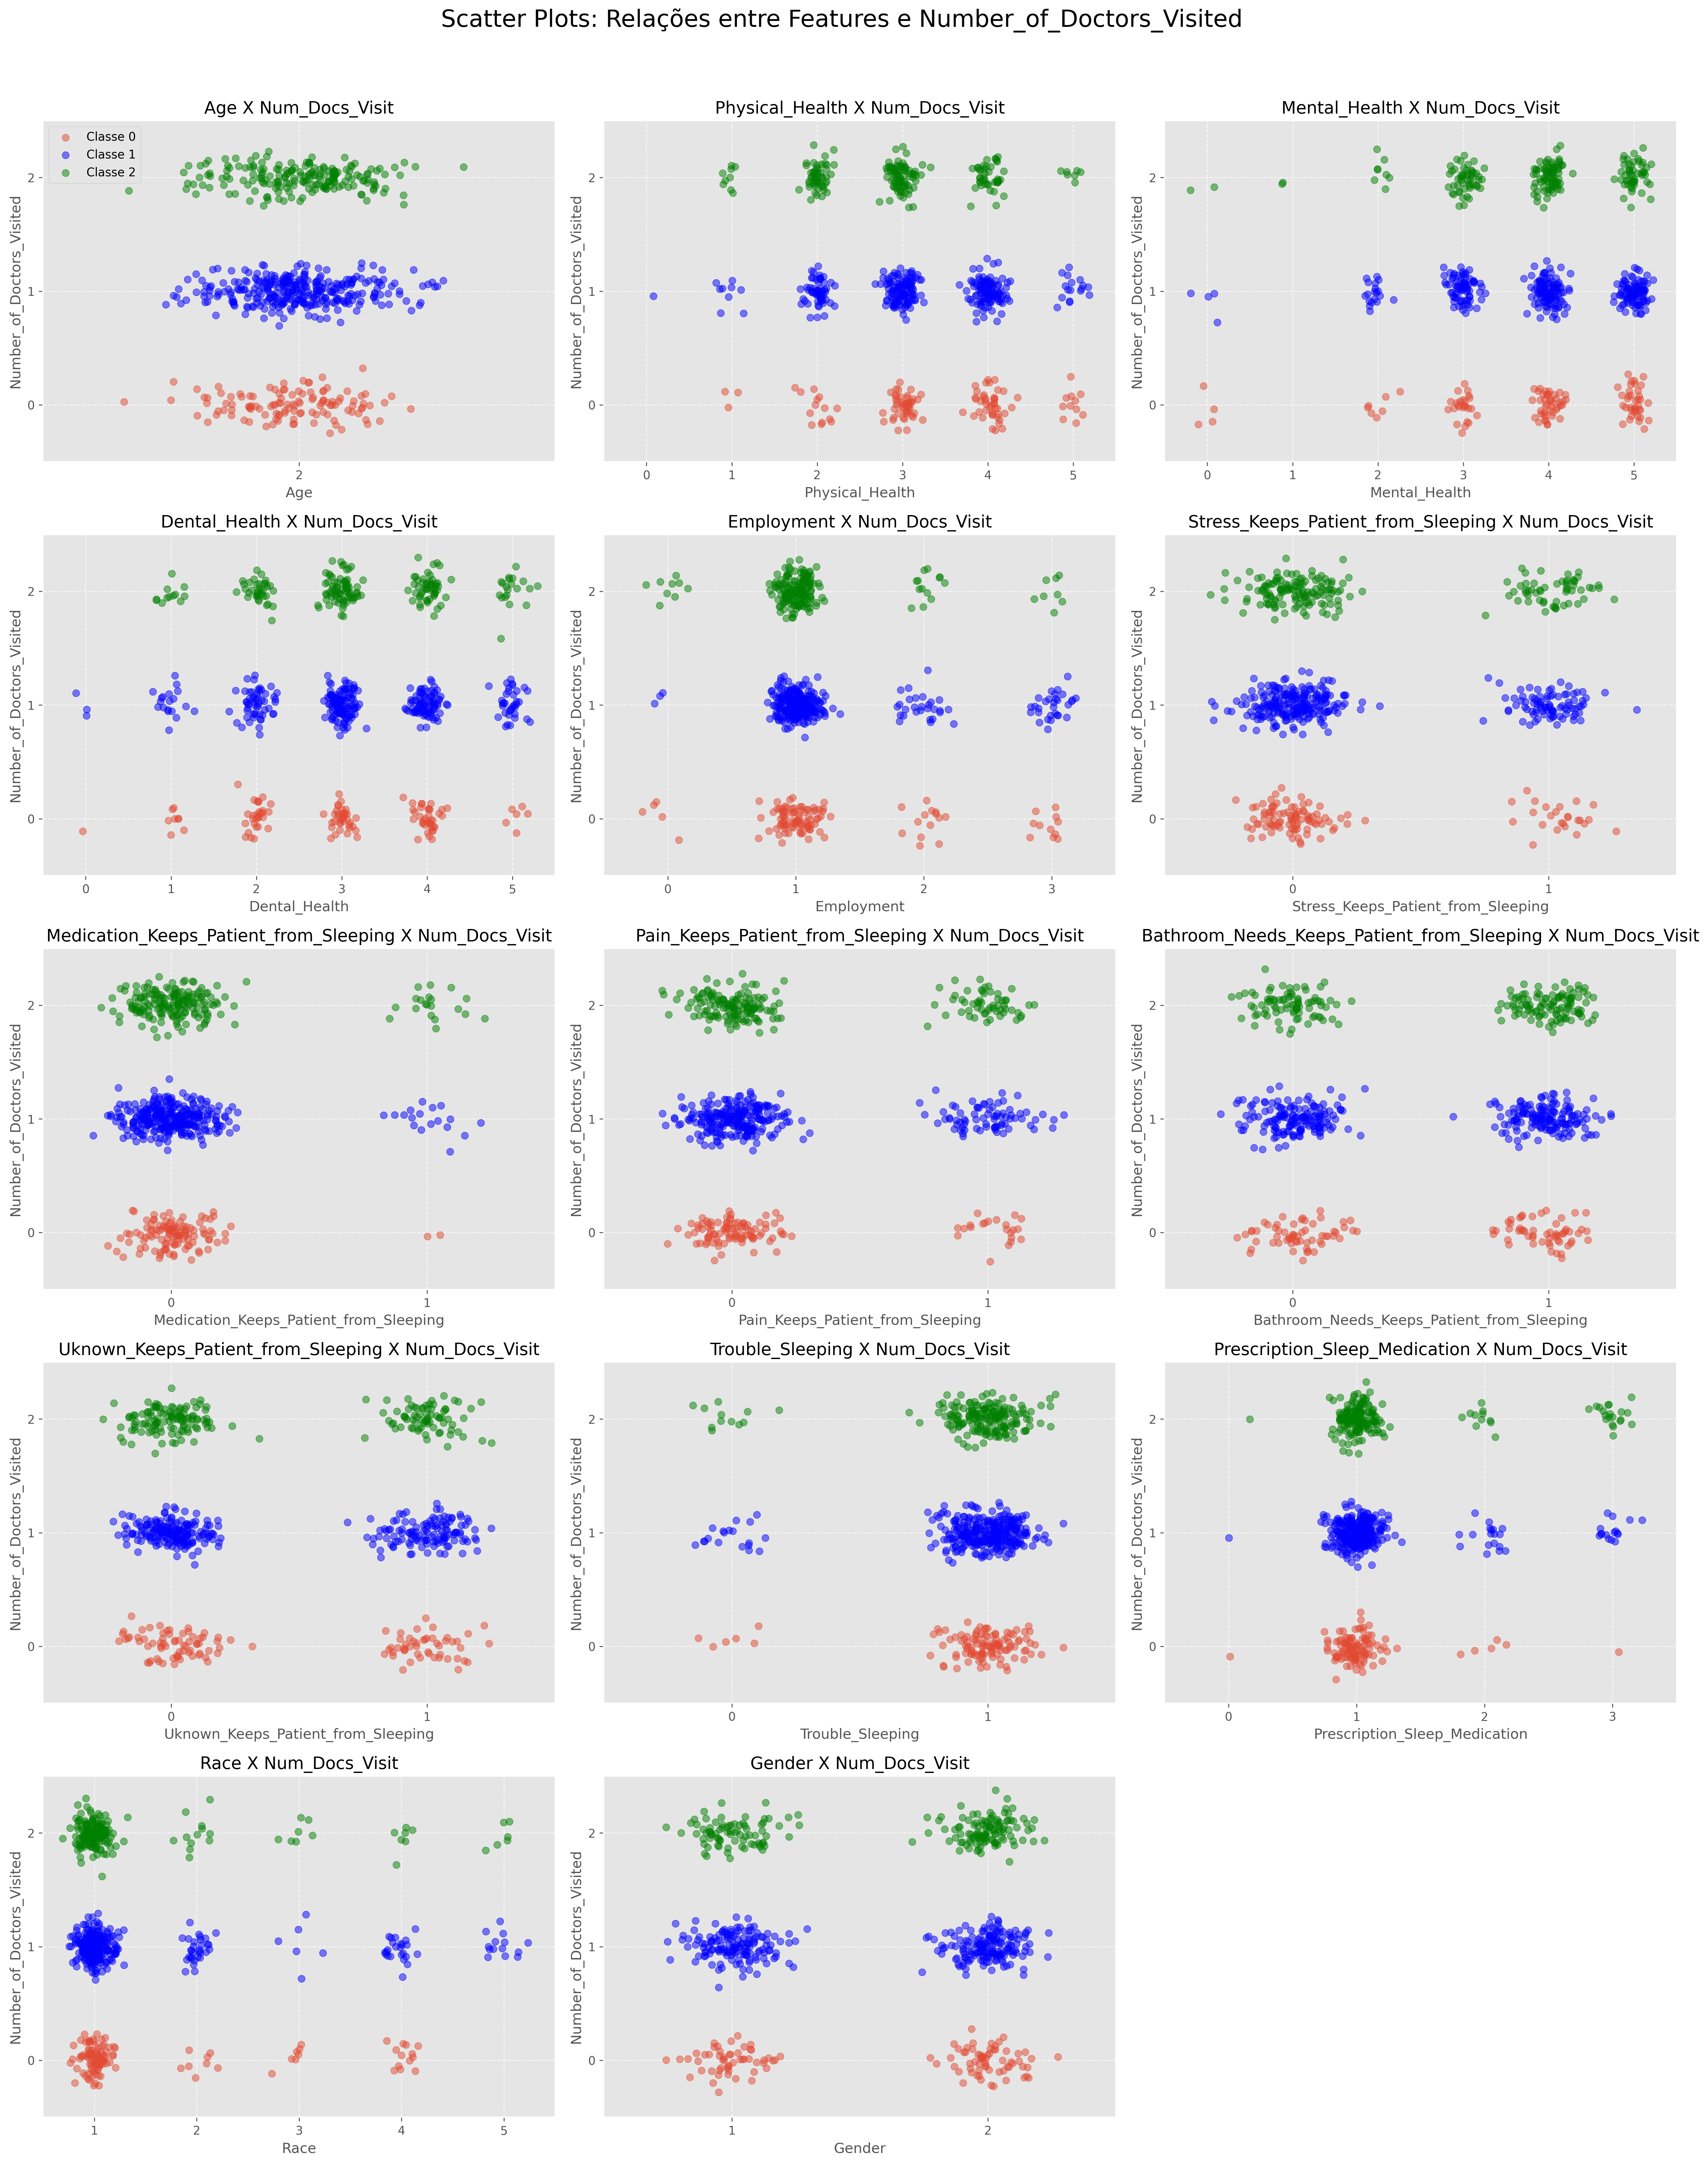
\includegraphics[width=\textwidth]{images/scatter_plot_mosaic.png}
    \caption{Análise de Relações Bivariadas: Mosaico de Gráficos de Dispersão entre Atributos Preditores e a Variável-Alvo (\textit{Number of Doctors Visited}). Pontos coloridos por classe: Vermelho (0-1 visita), Azul (2-3 visitas), Verde (4+ visitas).} % Legenda Aprimorada
    \label{fig:mosaico_dispersao}
\end{figure}

A análise do mosaico de gráficos de dispersão (Figura~\ref{fig:mosaico_dispersao}), onde as cores representam as classes da variável-alvo (vermelho: 0-1, azul: 2-3, verde: 4+ visitas), sugere as seguintes associações:

\begin{itemize}
    \item \textbf{Relações com Estado de Saúde} (\textit{Physical}, \textit{Mental}, \textit{Dental Health}): Observa-se uma associação inversa consistente; pior autoavaliação de saúde está associada a maior frequência de visitas (mais pontos verdes/azuis em valores baixos de saúde). \textit{Physical Health} aparenta ter a relação mais forte.
    
    \item \textbf{Fatores Relacionados ao Sono}:
    \begin{itemize}
        \item \textit{Stress}, \textit{Pain Keeps Patient from Sleeping}: Indivíduos que reportam esses problemas (valor 1) concentram-se mais na categoria de alta utilização (verde). A associação com dor parece particularmente expressiva.
        \item \textit{Prescription Sleep Medication}: Uso regular (valor 3) associa-se a maior frequência de visitas, enquanto não-usuários (valor 1) predominam na categoria de menor frequência.
        \item \textit{Trouble Sleeping}: Apesar da alta prevalência geral, dificuldades mais acentuadas parecem correlacionadas com maior utilização.
    \end{itemize}
    
    \item \textbf{Fatores Sociodemográficos}:
    \begin{itemize}
        \item \textit{Employment}: Trabalho integral (valor 3) associa-se a menor utilização, talvez por melhor saúde ou restrições de tempo.
        \item \textit{Race}, \textit{Gender}: Não mostram padrões claros de variação na frequência de visitas entre seus diferentes grupos/valores neste \textit{dataset}.
    \end{itemize}
\end{itemize}

Essas visualizações indicam que autoavaliação de saúde e distúrbios do sono (especialmente dor e uso de medicação) são preditores potenciais mais fortes que fatores sociodemográficos para a frequência de visitas médicas nesta amostra.

% Figura 3 - Legenda Aprimorada
\begin{figure}[htbp]
    \centering
    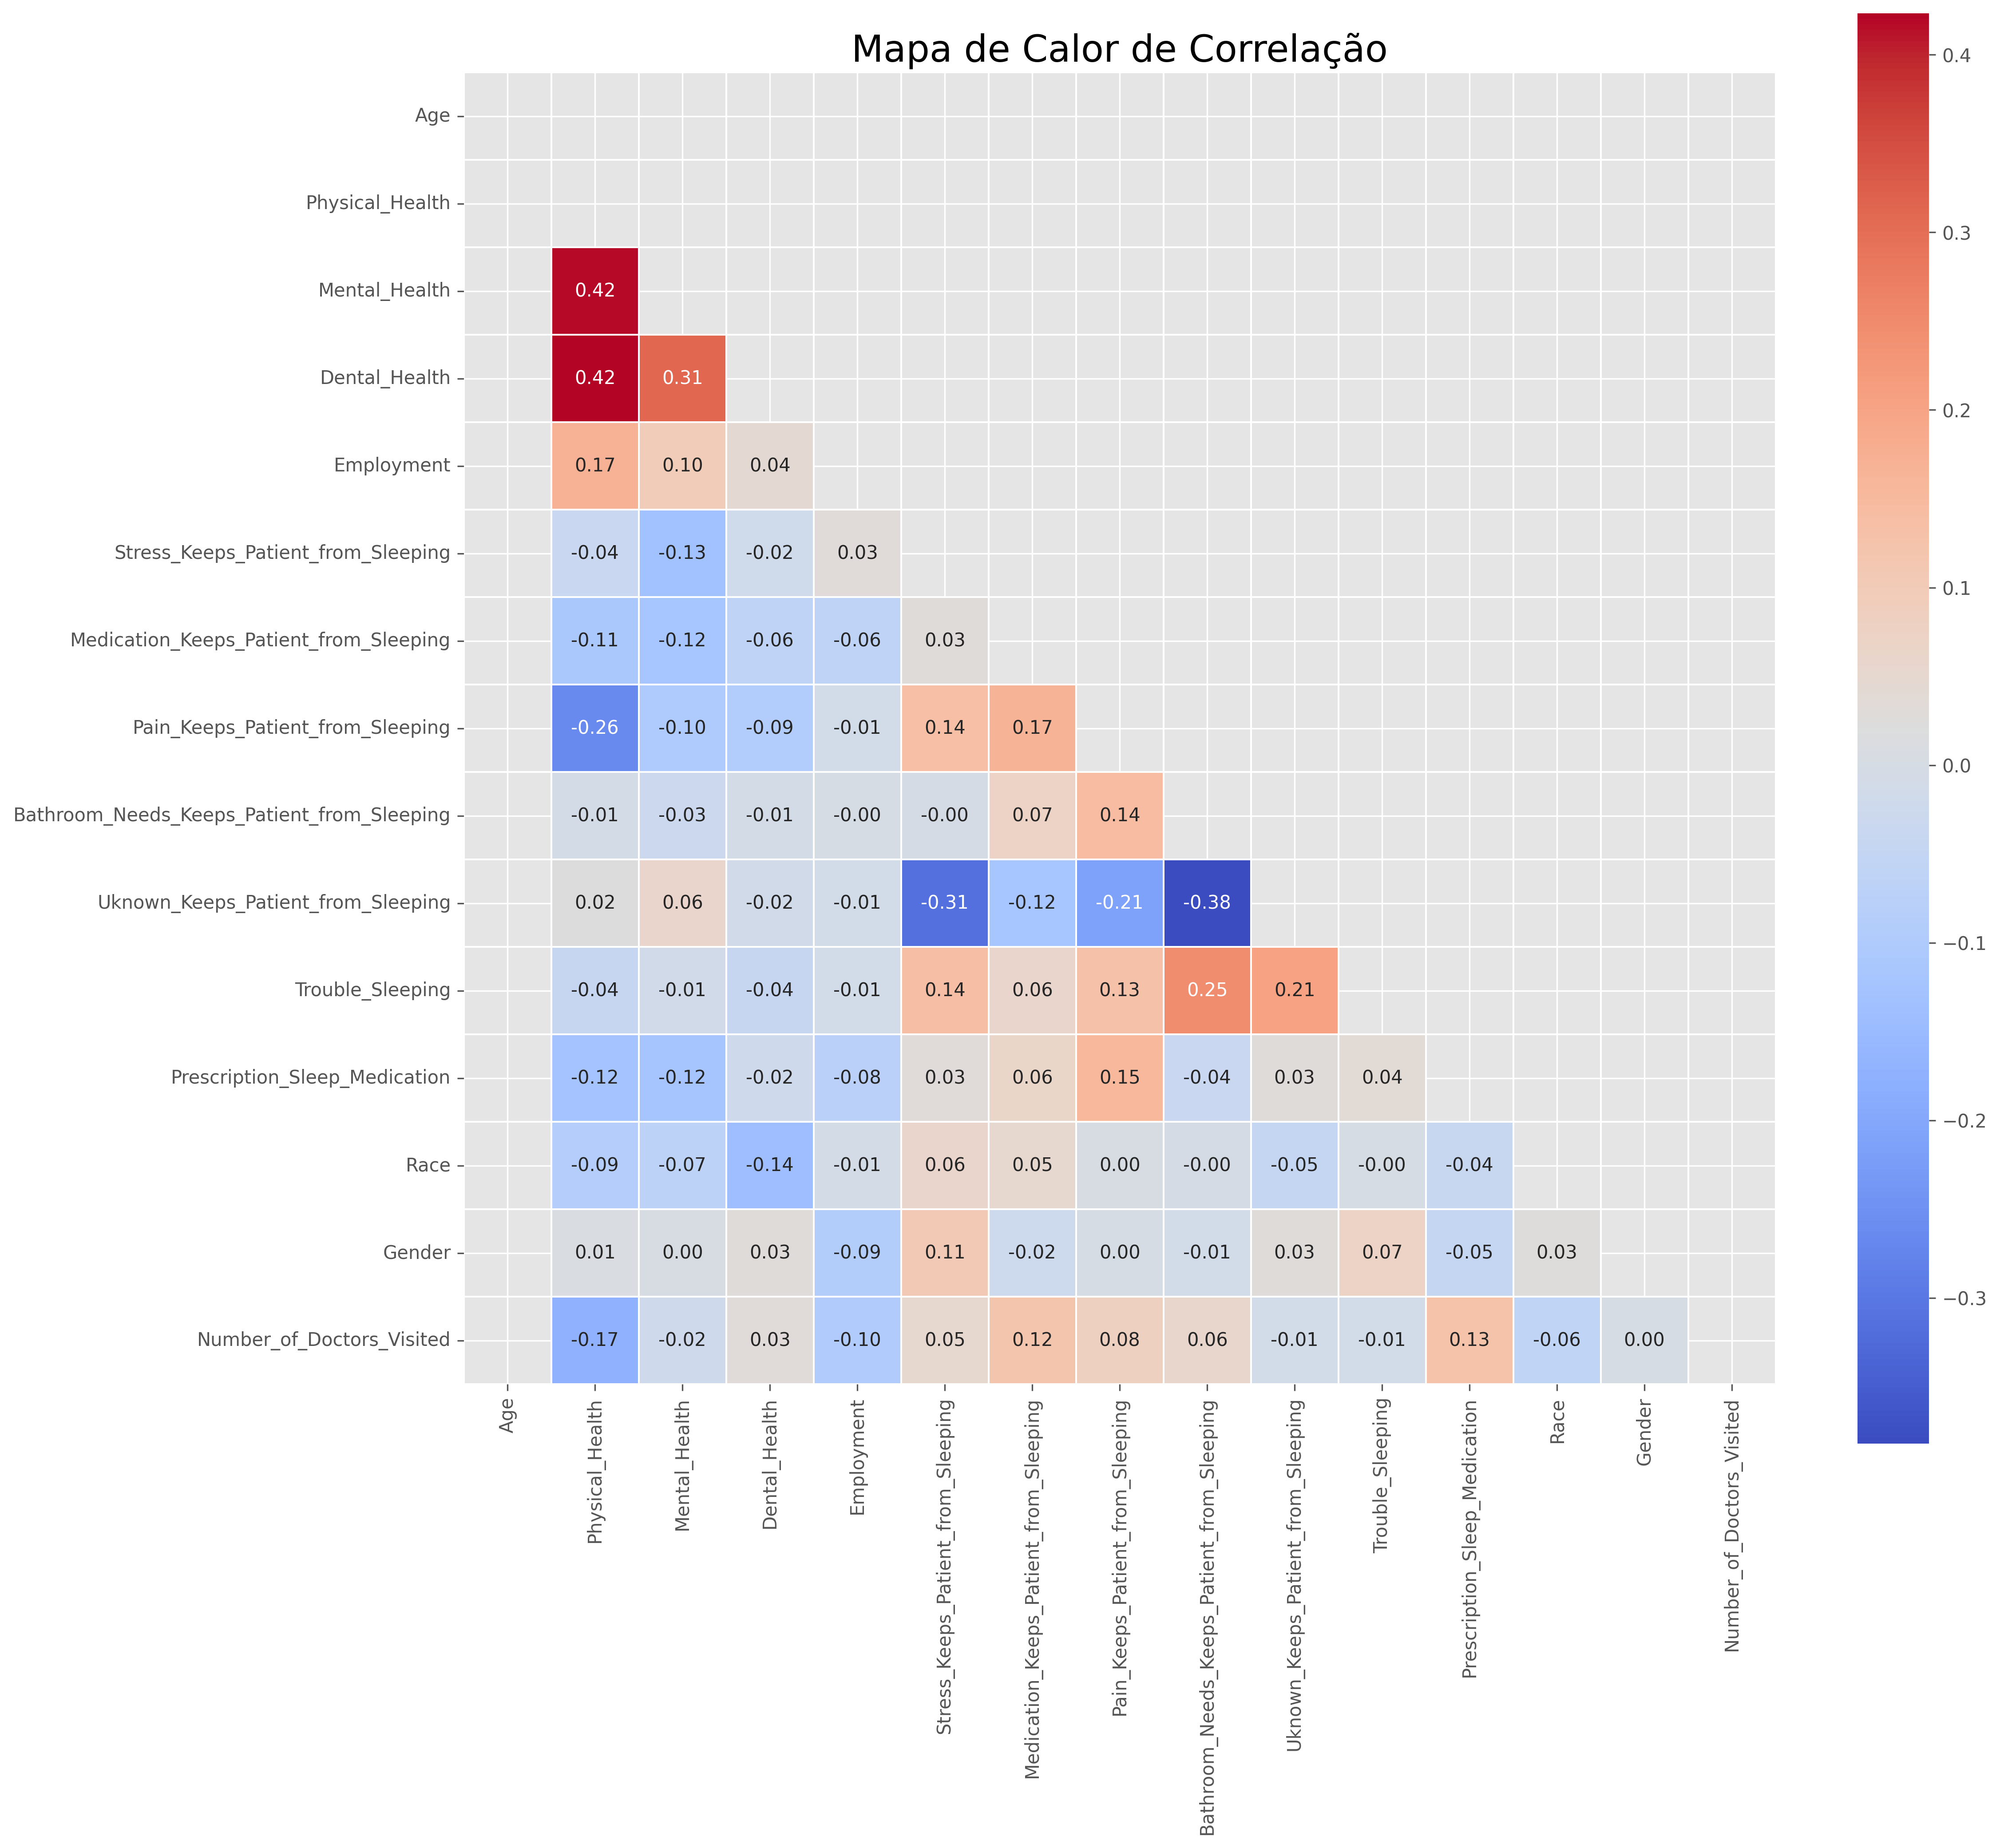
\includegraphics[width=\textwidth]{images/correlation_heatmap.png}
    \caption{Mapa de Calor das Correlações de Spearman: Intensidade e Direção das Associações Monotônicas entre Todos os Atributos do \textit{Dataset}} % Legenda Aprimorada
    \label{fig:mapa_correlacoes} 
\end{figure}

\subsubsection{Análise Quantitativa das Correlações} 

O mapa de calor (Figura~\ref{fig:mapa_correlacoes}), usando a correlação de Spearman \cite{hauke2011comparison}, quantifica as relações monotônicas:

\begin{itemize}
    \item \textbf{Correlações Mais Significativas com \textit{Number of Doctors Visited}}:
    \begin{itemize}
        \item \textit{Physical\_Health} (\textbf{-0,174}): A correlação negativa mais forte, confirmando que pior saúde física se associa a mais visitas \cite{Maaten2008}.
        \item \textit{Prescription\_Sleep\_Medication} (\textbf{+0,126}): A correlação positiva mais forte, ligando uso de medicação para dormir a mais visitas (possivelmente por necessidade de prescrição).
        \item \textit{Medication\_Keeps\_Patient\_from\_Sleeping} (+0,121): Associação positiva, talvez refletindo efeitos adversos que necessitam acompanhamento.
        \item \textit{Employment} (-0,097): Correlação negativa sugere que aposentados/sem trabalho visitam mais, talvez por disponibilidade ou condições de saúde \cite{Ahs2012}.
    \end{itemize}
    
    \item \textbf{Correlações Surpreendentemente Baixas}:
    \begin{itemize}
        \item \textit{Mental\_Health} (-0,021): Quase nula. Possíveis razões: subnotificação por estigma \cite{GONCALVES2014393}, fragmentação dos serviços de saúde mental, viés amostral (cuidadores), tratamento estabilizado.
        \item \textit{Dental\_Health} (+0,030): Magnitude negligenciável. Possíveis razões: atendimento odontológico separado (não contado na variável-alvo), priorização de outras condições, barreiras de acesso a planos odontológicos.
        \item \textit{Trouble\_Sleeping} (-0,013): Quase nula. Possíveis razões: inconsistências na codificação original (corrigida no pré-processamento), maior relevância da causa específica do distúrbio (dor, medicação) do que do sintoma geral, normalização do problema por idosos \cite{Lindstrom2012}.
    \end{itemize}
\end{itemize}

A análise quantitativa reforça a relevância de \textit{Physical Health} e \textit{Prescription Sleep Medication}. As correlações baixas para variáveis como \textit{Mental Health} e \textit{Dental Health} levantam hipóteses sobre fatores contextuais e limitações da variável-alvo, enriquecendo a compreensão do fenômeno.

\subsection{Pré-processamento e Tratamento dos Dados} 

O \textit{dataset} original não possuía valores ausentes. Foram removidas 83 instâncias duplicadas, resultando em 631 instâncias únicas.

Implementou-se uma padronização para variáveis ordinais de autoavaliação (\textit{Physical}, \textit{Mental}, \textit{Dental Health}), recodificando a escala original \{-1, 1, 2, 3, 4, 5\} para \{0 (recusa), 5 (ruim), 4 (regular), 3 (boa), 2 (muito boa), 1 (excelente)\}, onde 1 passa a representar a melhor avaliação. A variável-alvo (\textit{Number of Doctors Visited}) foi remapeada de \{1, 2, 3\} para \{0, 1, 2\} para compatibilidade com bibliotecas como \textit{scikit-learn}.

Inconsistências foram tratadas:
\begin{itemize}
    \item \textit{Dental Health}: Valores atípicos (6) foram substituídos pela mediana (3), melhorando ligeiramente a correlação com a variável-alvo.
    \item \textit{Trouble Sleeping}: Originalmente descrita como binária, mas continha valores \{-1, 1, 2, 3\}. Foi recodificada para binária (1 se qualquer variável específica de problema de sono fosse 1, 0 caso contrário), preservando a informação de forma conceitualmente coerente.
\end{itemize}

Não foram aplicadas normalização ou padronização estatística adicionais, dada a natureza predominantemente ordinal dos dados e a uniformidade escalar após o tratamento, preservando a interpretabilidade.

\subsection{Estratégia de Amostragem e Validação} 

% Figura 4 - Legenda Aprimorada
\begin{figure}[htbp]
    \centering
    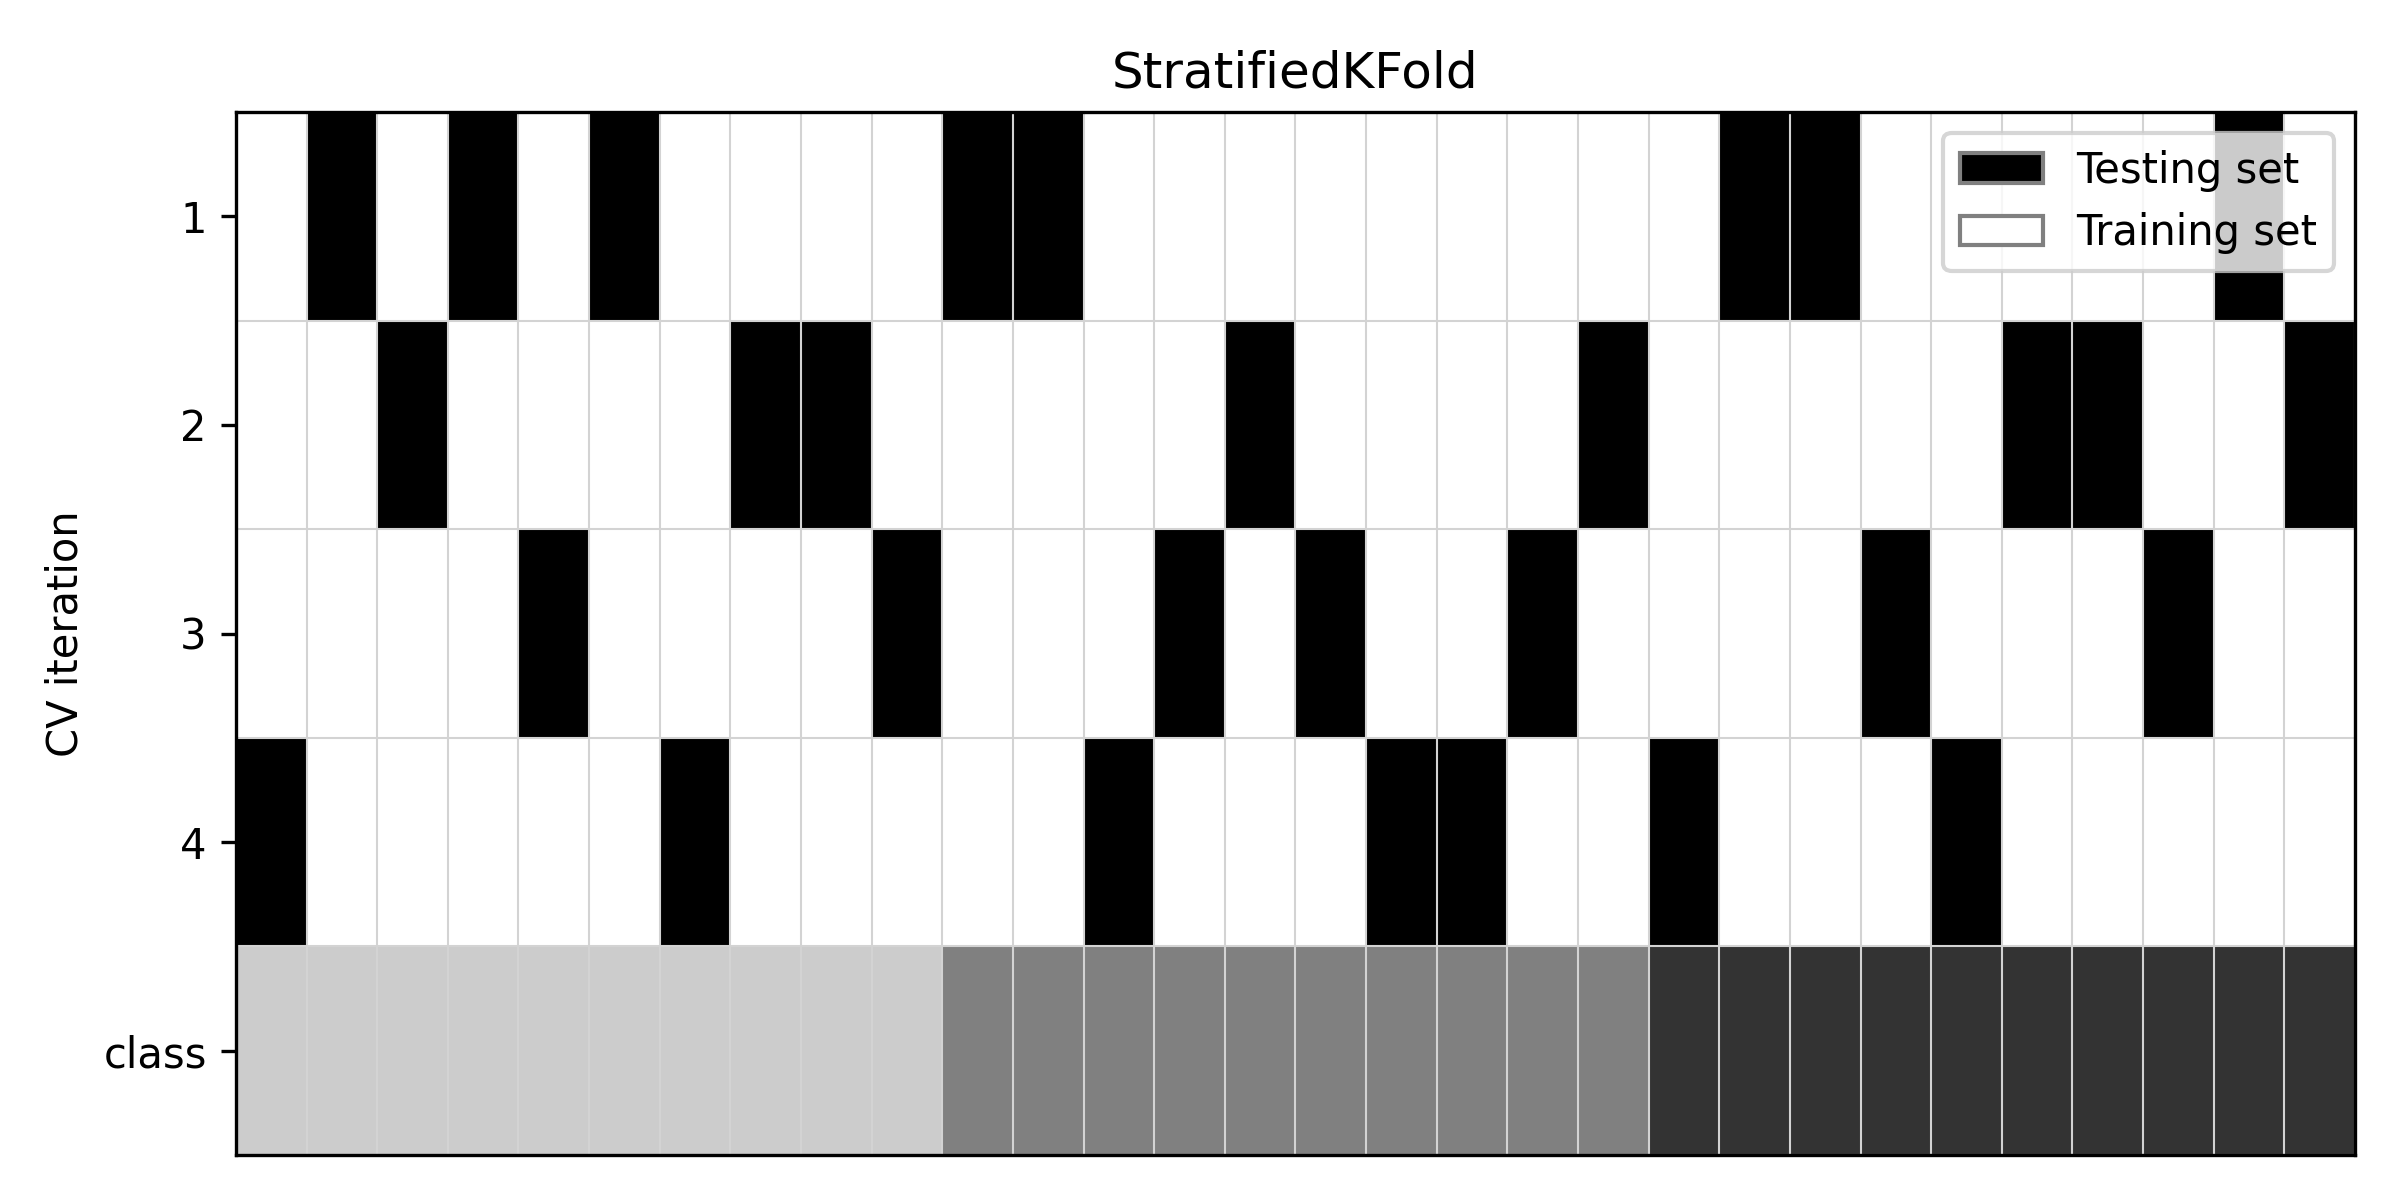
\includegraphics[width=\textwidth]{images/stratified_kfold_bw.png}
    \caption{Ilustração da Validação Cruzada Estratificada (\textit{StratifiedKFoldCV}) com k=4: Demonstração da divisão do \textit{dataset} em partições de treino (branco) e teste (preto), preservando a proporção das classes (faixas inferiores).} % Legenda Aprimorada
    \label{fig:stratifiedKFold}
\end{figure}

Adotou-se validação cruzada estratificada (\textit{StratifiedKFoldCV}) com $k = 5$ (Figura~\ref{fig:stratifiedKFold}), adequada para o tamanho do \textit{dataset} ($N=631$) \cite{Szeghalmy2023, CienciaDadosFund}. Cada uma das 5 partições (\textit{folds}) foi dividida em: 64\% para treinamento, 16\% para validação (otimização de hiperparâmetros) e 20\% para teste final.

A estratificação garante a manutenção da proporção das classes da variável-alvo em todas as divisões \cite{Szeghalmy2023}, crucial devido ao desbalanceamento observado. A avaliação em múltiplos \textit{folds} fornece métricas mais confiáveis e reduz o viés de amostragem comparado a uma divisão única (\textit{hold-out}) \cite{CienciaDadosFund}.

Para investigar o impacto do desbalanceamento, geramos 5 partições adicionais aplicando a técnica \textit{SMOTE} (\textit{Synthetic Minority Over-sampling Technique}) \cite{chawla2002smote} na porção de treinamento de cada \textit{fold}, permitindo uma análise comparativa do desempenho em cenários com e sem balanceamento sintético.

\subsection{Seleção de Atributos}

Implementamos um processo de seleção de atributos para identificar um subconjunto ótimo visando maximizar o desempenho preditivo. Testes preliminares indicaram que usar os 7 atributos com maior correlação superava usar todos os 14. Para sistematizar, aplicamos três abordagens (descritas no Algoritmo~\ref{alg:selecao_atributos}):

\begin{enumerate}
    \item \textbf{Limiar de Variância (\textit{Variance Threshold})}: Elimina atributos com variância abaixo de um limiar, pois baixa variabilidade oferece pouca informação discriminativa.
    \item \textbf{Seleção Univariada}: Avalia a relação estatística de cada atributo com a variável-alvo.
    \begin{itemize}
        \item \textbf{Teste Qui-Quadrado ($\chi^2$)}: Para atributos categóricos, seleciona aqueles com maior dependência estatística em relação à variável-alvo (maior $\chi^2$, menor p-valor).
        \item \textbf{Teste \textit{ANOVA} (F-test)}: Para atributos numéricos vs. alvo categórico, seleciona aqueles cujas médias diferem significativamente entre as classes (maior F, menor p-valor).
    \end{itemize}
\end{enumerate}

O Algoritmo~\ref{alg:selecao_atributos} detalha o processo: iteramos sobre diferentes números de atributos ($k$) para Qui-Quadrado e \textit{ANOVA}, e diferentes limiares para \textit{Variance Threshold}. Para cada subconjunto resultante, avaliamos o desempenho médio (usando validação cruzada interna) de todos os classificadores base, medido pela média geométrica do \textit{f1-score} ponderado ($m_1$) e \textit{roc auc score} ($m_2$) médios ($m_g = \sqrt{m_1 \cdot m_2}$). O subconjunto que maximizou $m_g$ foi selecionado.

% Algoritmo 1 - Legenda Aprimorada
\begin{adjustbox}{width=\textwidth}
\begin{algorithm}[H]
\footnotesize
\SetInd{0.5em}{0.5em}
\SetAlgoLined
\KwIn{$X$: \textit{dataset}\\
      $y$: variável-alvo\\
      $classificadores$: conjunto de classificadores\\
      $n\_folds$: número de partições CV}
\KwOut{Melhor subconjunto de atributos}

$k\_range \leftarrow [6, 7, ..., 15]$ 
$thresholds \leftarrow [0.0, 0.01, ..., 0.2]$ 
$resultados \leftarrow [ ]$\\

\ForEach{$metodo \in [ANOVA, Qui\text{-}Quadrado, VarianceThreshold]$}{
    \eIf{$metodo \in [ANOVA, Qui\text{-}Quadrado]$}{
        \ForEach{$k \in k\_range$}{
            $atributos\_selecionados \leftarrow \textsc{AplicaSeletor}(metodo, X, y, k)$\\
            $X_{sub} \leftarrow X[atributos\_selecionados]$\\
            
            $m_f \leftarrow 0$, $m_{auc} \leftarrow 0$\\
            \ForEach{$classificador \in classificadores$}{
                $scores \leftarrow \textsc{ValidacaoCruzada}(classificador, X_{sub}, y, n\_folds)$\\
                $m_f \leftarrow m_f + \text{media}(scores.\textit{f1\_score\_weighted})$\\ 
                $m_{auc} \leftarrow m_{auc} + \text{media}(scores.\textit{roc\_auc\_score})$\\ 
            }
            
            $m_1 \leftarrow m_f / |\text{classificadores}|$\\
            $m_2 \leftarrow m_{auc} / |\text{classificadores}|$\\
            $m_g \leftarrow \sqrt{m_1 \cdot m_2}$\\
            
            $resultados.\textsc{Adicionar}(\{m_g, metodo, k, atributos\_selecionados\})$\\
        }
    }{% Else (VarianceThreshold)
        \ForEach{$threshold \in thresholds$}{
            $atributos\_selecionados \leftarrow \textsc{AplicaVariancia}(X, threshold)$\\
            $X_{sub} \leftarrow X[atributos\_selecionados]$\\
            
            $m_f \leftarrow 0$, $m_{auc} \leftarrow 0$\\
            \ForEach{$classificador \in classificadores$}{
                $scores \leftarrow \textsc{ValidacaoCruzada}(classificador, X_{sub}, y, n\_folds)$\\
                $m_f \leftarrow m_f + \text{media}(scores.\textit{f1\_score\_weighted})$\\ 
                $m_{auc} \leftarrow m_{auc} + \text{media}(scores.\textit{roc\_auc\_score})$\\ 
            }
            
            $m_1 \leftarrow m_f / |\text{classificadores}|$\\
            $m_2 \leftarrow m_{auc} / |\text{classificadores}|$\\
            $m_g \leftarrow \sqrt{m_1 \cdot m_2}$\\
            
            $resultados.\textsc{Adicionar}(\{m_g, metodo, threshold, atributos\_selecionados\})$\\
        }
    }
}

$melhor\_resultado \leftarrow \underset{r \in resultados}{\operatorname{argmax}}(r.m_g)$\\
\KwRet{$melhor\_resultado.atributos\_selecionados$}
\caption{Algoritmo para Seleção de Atributos: Combinação de Métodos (\textit{ANOVA}, Qui-Quadrado, \textit{Variance Threshold}) para Identificar o Subconjunto Preditivo Ótimo} % Legenda Aprimorada
\label{alg:selecao_atributos} 
\end{algorithm}
\end{adjustbox}

Os atributos selecionados foram: \textit{Physical Health}, \textit{Dental Health}, \textit{Employment}, \textit{Prescription Sleep Medication}, \textit{Race} e \textit{Gender}.

\subsection{Otimização de Hiperparâmetros} 

Utilizamos o \textit{framework} Optuna \cite{akiba2019optuna} para otimização de hiperparâmetros, empregando busca adaptativa (TPE). Funções objetivo específicas foram criadas para cada classificador, avaliando configurações nos \textit{folds} de validação (16\% de cada partição estratificada).

Definimos espaços de busca personalizados (Tabela~\ref{tab:hiperparametros}) para os hiperparâmetros mais influentes de cada modelo.

% Tabela 3 - Legenda Aprimorada
\begin{table}[htbp]
\centering
\scriptsize 
\caption{Espaços de Busca para Otimização de Hiperparâmetros com Optuna: Intervalos e Valores Considerados para Cada Algoritmo de Classificação} % Legenda Aprimorada
\label{tab:hiperparametros}
\begin{tabularx}{\textwidth}{|p{2.2cm}|X|} 
\hline
\textbf{Algoritmo} & \textbf{Hiperparâmetros (Intervalo/Valores)} \\
\hline
\textit{Decision Trees} & max\_depth (3-30); min\_samples\_split (2-20); min\_samples\_leaf (1-10); criterion \{\textit{gini}, \textit{entropy}\} \\ 
\hline
\textit{Gradient Tree Boosting} & n\_estimators (50-500); learning\_rate (0.01-0.3); max\_depth (3-10); min\_samples\_split (2-20); min\_samples\_leaf (1-10); subsample (0.6-1.0) \\
\hline
\textit{k-Nearest Neighbors} & n\_neighbors (1-30); weights \{\textit{uniform}, \textit{distance}\}; algorithm \{\textit{auto}, \textit{ball\_tree}, \textit{kd\_tree}, \textit{brute}\}; p \{1, 2\} (Manhattan, Euclidiana) \\ 
\hline
\textit{Multinomial Logistic Regression} & C (10$^{-4}$-10$^{2}$); solver \{\textit{newton-cg}, \textit{lbfgs}, \textit{sag}, \textit{saga}\} \\ 
\hline
\textit{Naive Bayes} & var\_smoothing (10$^{-12}$-10$^{-2}$) \\
\hline
\textit{Random Forests} & n\_estimators (50-500); max\_depth (3-30); min\_samples\_split (2-20); min\_samples\_leaf (1-10); bootstrap \{\textit{True}, \textit{False}\}; criterion \{\textit{gini}, \textit{entropy}\} \\ 
\hline
\textit{Support Vector Machines} & C (10$^{-4}$-10$^{2}$); kernel \{\textit{linear}, \textit{poly}, \textit{rbf}, \textit{sigmoid}\}; gamma \{\textit{scale}, \textit{auto}\} \\ 
\hline
XGBoost & n\_estimators (50-500); learning\_rate (0.01-0.3); max\_depth (3-12); min\_child\_weight (1-10); subsample (0.6-1.0); colsample\_bytree (0.6-1.0) \\
\hline
LightGBM & n\_estimators (50-500); learning\_rate (0.01-0.3); num\_leaves (20-100); max\_depth (3-12); min\_child\_samples (5-100); subsample (0.6-1.0); colsample\_bytree (0.6-1.0) \\
\hline
CatBoost & iterations (50-500); learning\_rate (0.01-0.3); depth (4-10); l2\_leaf\_reg (10$^{-8}$-10); bagging\_temperature (0-10); grow\_policy \{\textit{SymmetricTree}, \textit{Depthwise}, \textit{Lossguide}\} \\ 
\hline
\end{tabularx}
\end{table}

Realizamos 50 tentativas por modelo, otimizando o \textit{f1-score} ponderado médio nos \textit{folds} de validação. A estratégia do Optuna direciona a busca eficientemente. Os melhores conjuntos de hiperparâmetros encontrados foram usados para treinar os modelos finais nos dados de treinamento (64\% de cada partição) para avaliação nos dados de teste (20\%). Este processo sistemático elevou o desempenho de todos os classificadores em comparação com suas configurações padrão.

\subsection{Avaliação dos Modelos}

\subsubsection{Comparação Estatística} 

Adotamos a metodologia de Demšar (2006) \cite{demsarStatistical} para comparar o desempenho relativo dos 13 classificadores (incluindo os 3 DES), identificando diferenças estatisticamente significativas e evitando conclusões baseadas em variações aleatórias.

Utilizamos testes não paramétricos em duas etapas:
\begin{enumerate}
    \item \textbf{Teste de Friedman}: Avalia $H_0$ de que todos os classificadores têm desempenho equivalente (\textit{f1-score} ponderado). Usa rankings por \textit{fold} e a estatística $F_F$ (Eq. 1 e 2) com $N=5, k=13$.
    \item \textbf{Teste Post-hoc de Nemenyi}: Se $H_0$ for rejeitada ($\alpha=0.05$), calcula a Diferença Crítica (CD) (Eq. 3) para identificar pares significativamente diferentes. $q_\alpha \approx 3.285$ para $k=13$.
\end{enumerate}
% Equações mantidas como antes

Os \textit{f1-scores} individuais foram obtidos avaliando os modelos otimizados nos 5 \textit{folds} de teste.

\subsubsection{Resultados da Comparação Estatística}

A Tabela~\ref{tab:performance_matrix} mostra os \textit{f1-scores} por \textit{fold} e a Tabela~\ref{tab:ranking_updated} os rankings médios.

% Tabela 4 - Legenda Aprimorada
\begin{table}[htbp]
    \centering
    \caption{Matriz de Desempenho Detalhada: Valores do \textit{F1-Score} Ponderado Obtidos por Cada Classificador em Cada uma das 5 Partições (\textit{Folds}) de Teste} % Legenda Aprimorada
    \label{tab:performance_matrix}
    \resizebox{\textwidth}{!}{
    \begin{tabular}{|c|ccccccccccccc|}
        \hline
        \textbf{Partição} & \textbf{DT} & \textbf{GB} & \textbf{k-NN} & \textbf{LGBM} & \textbf{LR} & \textbf{NB} & \textbf{RF} & \textbf{SVM} & \textbf{XGB} & \textbf{CAT} & \textbf{META} & \textbf{KNU} & \textbf{KNE} \\
        \hline
        0 & 0,3783 & 0,3711 & 0,4162 & 0,3988 & 0,4484 & 0,2577 & 0,4294 & 0,4354 & 0,3812 & 0,4027 & 0,4401 & 0,4250 & 0,4382 \\
        1 & 0,3881 & 0,3974 & 0,2576 & 0,3816 & 0,4492 & 0,2849 & 0,3721 & 0,3739 & 0,3897 & 0,3441 & 0,4075 & 0,3700 & 0,3711 \\
        2 & 0,3575 & 0,3262 & 0,3552 & 0,3497 & 0,4016 & 0,1580 & 0,3585 & 0,3663 & 0,3817 & 0,3472 & 0,3378 & 0,3492 & 0,3474 \\
        3 & 0,4391 & 0,3772 & 0,4106 & 0,4126 & 0,4706 & 0,4494 & 0,4644 & 0,4364 & 0,5300 & 0,3892 & 0,4519 & 0,4659 & 0,4579 \\
        4 & 0,2426 & 0,3707 & 0,2685 & 0,3391 & 0,3642 & 0,3237 & 0,3381 & 0,3517 & 0,3827 & 0,3597 & 0,3325 & 0,3594 & 0,3573 \\
        \hline
    \end{tabular}
    }
    \flushleft{\footnotesize{Abreviações: DT = \textit{Decision Trees}, GB = \textit{Gradient Boosting}, k-NN = \textit{k-Nearest Neighbors}, LGBM = LightGBM, LR = \textit{Logistic Regression}, NB = \textit{Naive Bayes}, RF = \textit{Random Forests}, SVM = \textit{Support Vector Machines}, XGB = XGBoost, CAT = CatBoost, META = META-DES, KNU = KNORA-Union, KNE = KNORA-Eliminate.}}
\end{table}

% Tabela 5 - Legenda Aprimorada e Bolding Mantido
\begin{table}[htbp]
    \centering
    \caption{Ranking Médio dos Classificadores: Classificação Geral Baseada no Desempenho Médio (\textit{F1-Score} Ponderado) ao Longo das 5 Partições de Teste} % Legenda Aprimorada
    \label{tab:ranking_updated}
    \resizebox{0.6\textwidth}{!}{ 
    \begin{tabular}{|l|c|}
        \hline
        \textbf{Classificador} & \textbf{Ranking Médio} \\
        \hline
        \textbf{\textit{Logistic Regression}} & \textbf{1,6} \\ 
        XGBoost & 3,6 \\
        \textit{Random Forest} & 6,0 \\ 
        \textit{SVM} & 6,0 \\ 
        METADES & 6,2 \\
        KNORAU & 6,4 \\
        KNORAE & 6,4 \\
        LightGBM & 8,0 \\
        \textit{Decision Tree} & 8,4 \\ 
        \textit{Gradient Boosting} & 8,4 \\ 
        CatBoost & 9,0 \\
        \textit{K-Nearest Neighbors} & 9,8 \\ 
        \textbf{\textit{Naive Bayes}} & \textbf{11,2} \\ 
        \hline
    \end{tabular}
    }
\end{table}

O teste de Friedman ajustado ($F_F = 3,0325, p = 0,003087$) rejeitou $H_0$, confirmando diferenças significativas. O teste de Nemenyi ($CD \approx 8,09$) mostrou que \textit{Logistic Regression} (Rank 1.6) foi significativamente superior a \textit{Naive Bayes} (Rank 11.2) e \textit{K-Nearest Neighbors} (Rank 9.8). Nenhuma outra diferença foi significativa.

\subsubsection{Visualização e Discussão dos Resultados} 

% Figura 5 - Legenda Aprimorada
\begin{figure}[htbp]
    \centering
    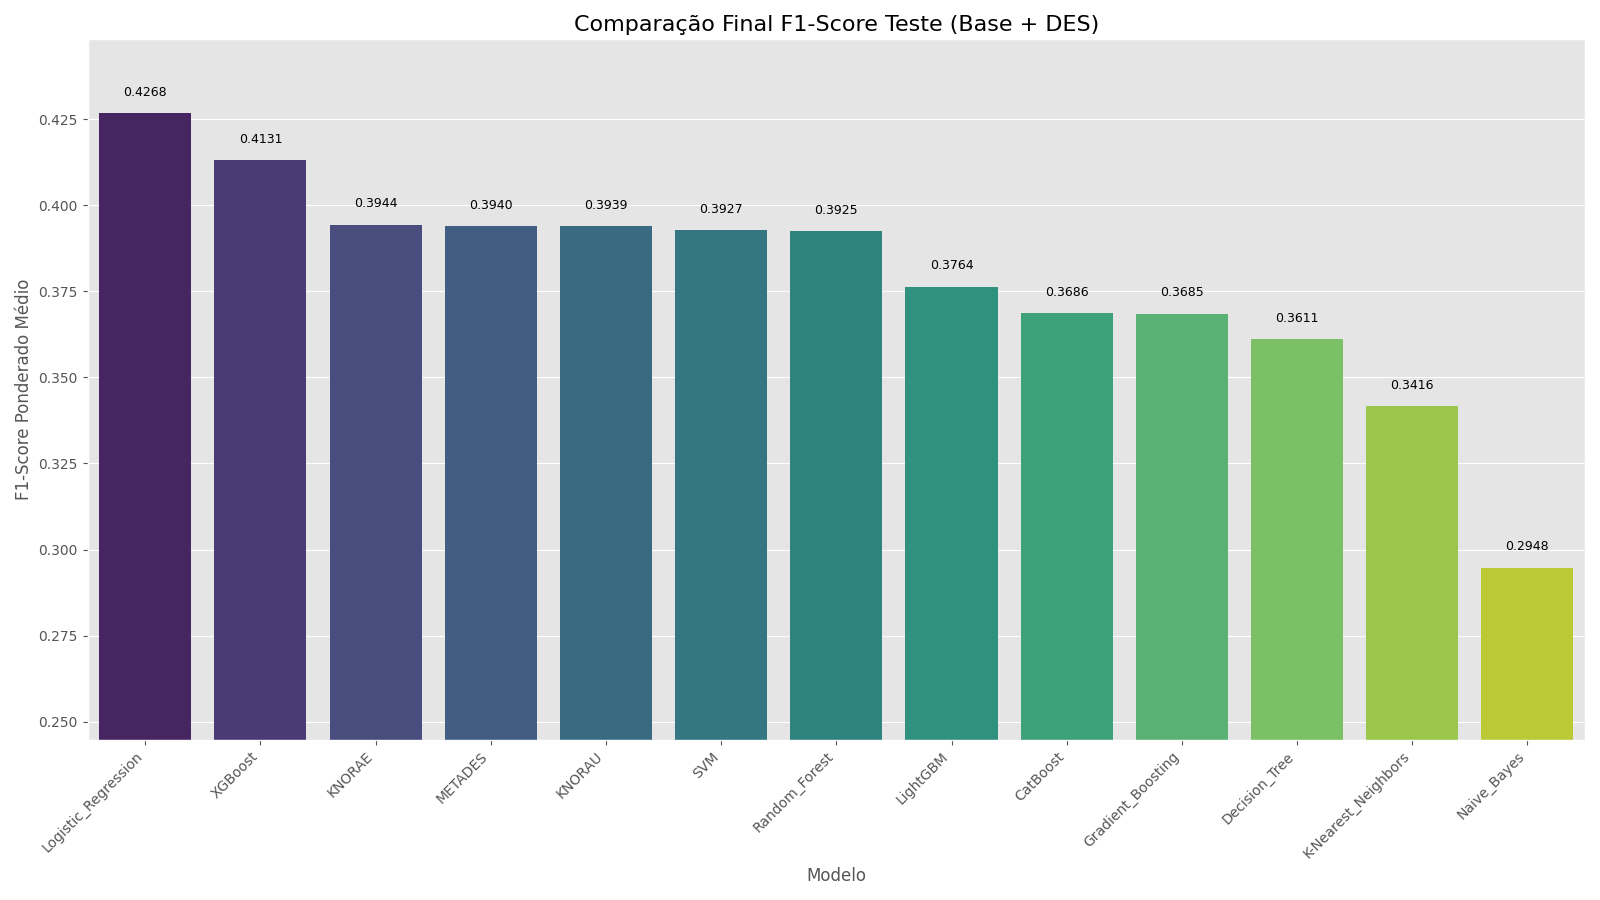
\includegraphics[width=0.9\textwidth]{images/models_test_evaluation.png}
    \caption{Visualização Comparativa do Desempenho Médio: \textit{F1-Score} Ponderado Médio Atingido por Cada Classificador no Conjunto de Teste (média das 5 partições)} % Legenda Aprimorada
    \label{fig:models_test_eval_driagram}
\end{figure}

A Figura~\ref{fig:models_test_eval_driagram} ilustra os \textit{f1-scores} médios. A análise estatística ($p=0.003$) e o teste de Nemenyi confirmam a superioridade de \textit{Logistic Regression} sobre NB e k-NN. Contudo, LR não diferiu estatisticamente de XGBoost, \textit{Random Forest}, \textit{SVM} e dos modelos DES, indicando um grupo de topo com desempenho similar, superior aos modelos de pior performance.

\subsection{Visualização da Curva de Perda para Modelos \textit{Boosting}} 

% Figuras 6, 7, 8 - Legendas Aprimoradas
\begin{figure}[htbp]
    \centering
    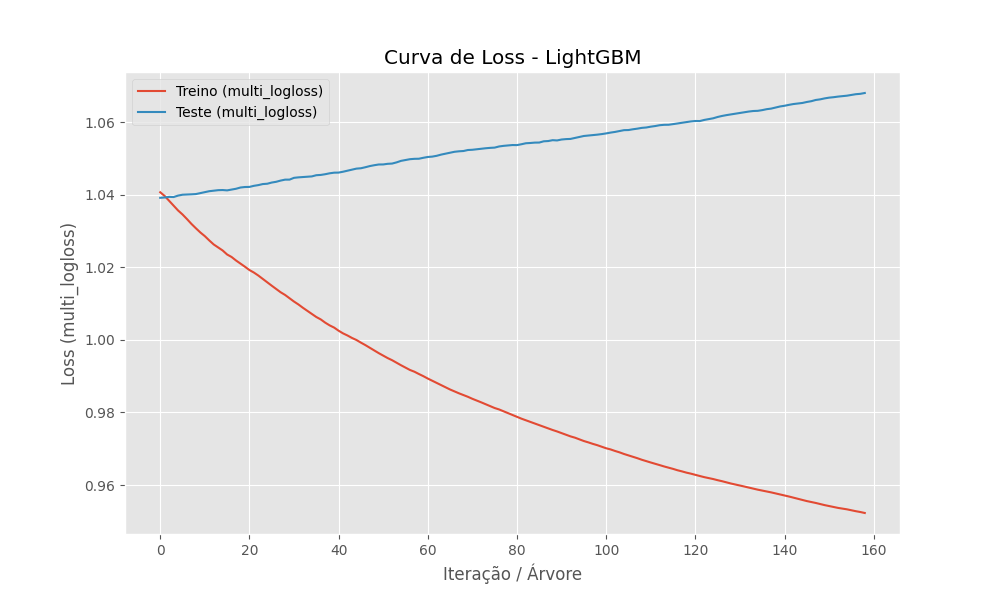
\includegraphics[width=0.9\textwidth]{images/loss_curve_LightGBM.png}
    \caption{Curvas de Aprendizagem para LightGBM: Evolução da Função de Perda (\textit{Multi-Logloss}) nos Conjuntos de Treinamento e Teste ao Longo das Iterações (\textit{Boosting Rounds})} % Legenda Aprimorada
    \label{fig:lighgbm_loss}
\end{figure}

\begin{figure}[htbp]
    \centering
    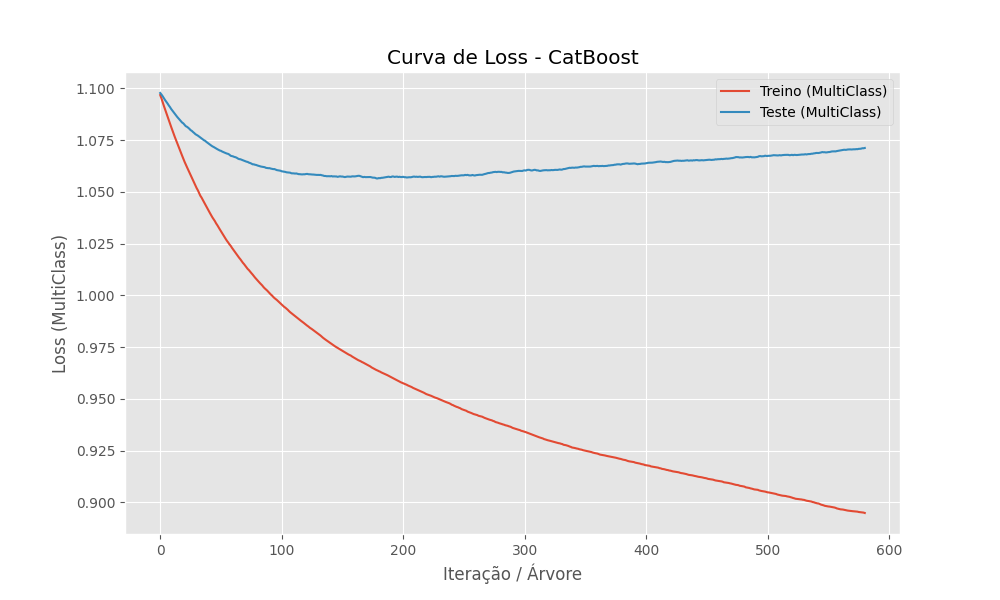
\includegraphics[width=0.9\textwidth]{images/loss_curve_CatBoost.png}
    \caption{Curvas de Aprendizagem para CatBoost: Evolução da Função de Perda (\textit{MultiClass}) nos Conjuntos de Treinamento e Teste ao Longo das Iterações (\textit{Boosting Rounds})} % Legenda Aprimorada
    \label{fig:catboost_loss}
\end{figure}

\begin{figure}[htbp]
    \centering
    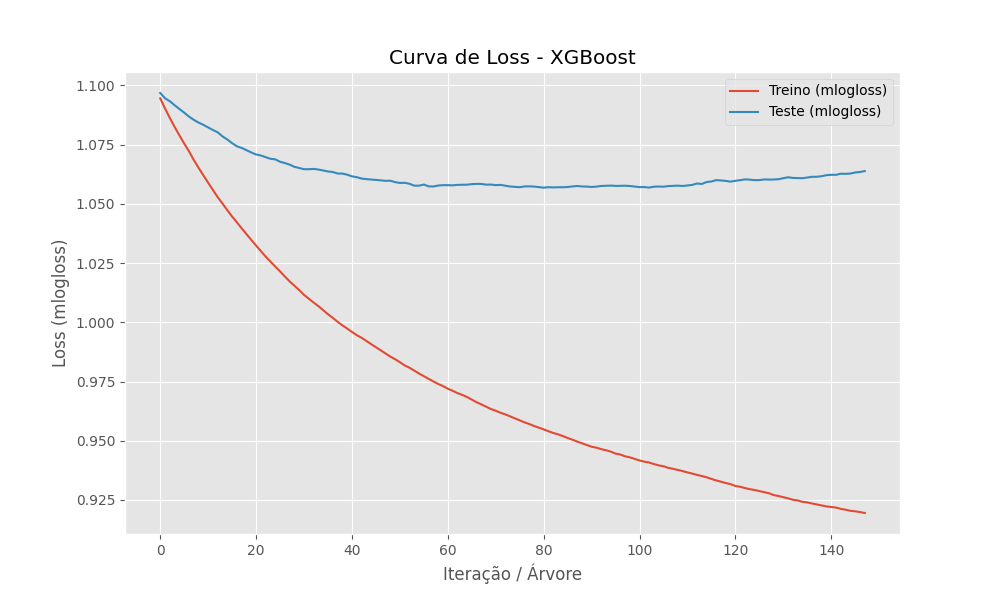
\includegraphics[width=0.9\textwidth]{images/loss_curve_XGBoost.png}
    \caption{Curvas de Aprendizagem para XGBoost: Evolução da Função de Perda (\textit{mlogloss}) nos Conjuntos de Treinamento e Teste ao Longo das Iterações (\textit{Boosting Rounds})} % Legenda Aprimorada
    \label{fig:xgboost_loss}
\end{figure}

Analisamos a evolução da função de perda (\textit{loss}) para LightGBM, CatBoost e XGBoost (Figuras~\ref{fig:lighgbm_loss}, \ref{fig:catboost_loss}, \ref{fig:xgboost_loss}).

LightGBM (Figura~\ref{fig:lighgbm_loss}) mostrou aumento da \textit{loss} no teste enquanto a \textit{loss} de treino diminuía, sugerindo dificuldade de generalização ou \textit{overfitting} inicial. CatBoost (Figura~\ref{fig:catboost_loss}) e XGBoost (Figura~\ref{fig:xgboost_loss}) exibiram padrões de \textit{overfitting}: \textit{loss} de treino decrescente, enquanto a \textit{loss} de teste estabilizava/aumentava após redução inicial, indicando perda de generalização com mais iterações.

% Seção 4: Conclusão (mantida como na versão anterior, com itálicos consistentes)
\section{Conclusão}
Este trabalho apresentou uma análise comparativa rigorosa de múltiplos classificadores – incluindo abordagens clássicas, \textit{boosting} e \textit{Dynamic Ensemble Selection} (DES) – para a modelagem preditiva da frequência de visitas médicas em indivíduos com 50+ anos, usando dados da NPHA \cite{NPHA2017}. Através de validação cruzada estratificada, otimização via Optuna \cite{akiba2019optuna}, e comparação estatística (Friedman/Nemenyi \cite{demsarStatistical}), identificamos diferenças significativas no desempenho dos modelos ($p=0.003$), apesar dos desafios de previsibilidade da tarefa.

\textit{Logistic Regression} alcançou o melhor desempenho médio (ranking 1.6), superando estatisticamente \textit{Naive Bayes} (11.2) e \textit{K-Nearest Neighbors} (9.8) ($CD \approx 8.09, \alpha=0.05$). Algoritmos como XGBoost e as técnicas DES (META-DES, KNORA-U, KNORA-E) mostraram-se competitivos, estatisticamente equivalentes ao melhor classificador. Este achado suporta a adequação de DES para \textit{datasets} limitados \cite{Cruz_2015, ICPRAI2018SI}. A análise também selecionou 6 atributos (\textit{Physical Health, Dental Health, Employment, Prescription Sleep Medication, Race, Gender}) com maior poder preditivo relativo.

Uma constatação central é a dificuldade intrínseca na predição da variável-alvo com alta acurácia neste \textit{dataset}. O tamanho amostral modesto ($N=631$) e as características dos dados limitaram o \textit{F1-Score} ponderado, mesmo após otimização. A análise das curvas de perda dos modelos de \textit{boosting} (Figuras~\ref{fig:lighgbm_loss}-\ref{fig:xgboost_loss}) reforçou a complexidade, evidenciando \textit{overfitting}. A não superioridade estatística do DES sobre \textit{Logistic Regression} pode derivar desses fatores, talvez exigindo otimização específica dos meta-parâmetros DES ou do \textit{pool} de classificadores.

Não obstante as limitações preditivas, as contribuições residem: (i) na aplicação e avaliação metodológica rigorosa de classificadores a um \textit{dataset} de saúde pública relevante (NPHA); (ii) na caracterização das limitações preditivas inerentes a este \textit{dataset} para a tarefa; (iii) na confirmação da competitividade de DES em cenários de dados limitados; e (iv) na identificação dos preditores mais relevantes.

\subsection*{Trabalhos Futuros}
Sugerem-se as seguintes direções:
\begin{itemize}
    \item \textbf{Enriquecimento e Validação de Dados:} Buscar amostras adicionais da NPHA ou integrar fontes longitudinais/clínicas para aumentar o poder estatístico. Validar/corrigir ruídos identificados nas variáveis.
    \item \textbf{Abordagens para Desbalanceamento e Baixa Performance:} Investigar sistematicamente técnicas avançadas de reamostragem ou algoritmos sensíveis ao custo para mitigar o desbalanceamento e melhorar as métricas absolutas.
    \item \textbf{Aprofundamento em Modelos DES:} Explorar estratégias heterogêneas para geração do \textit{pool} base. Realizar otimização dedicada dos hiperparâmetros DES e avaliar variantes robustas a dados desbalanceados \cite{ICPRAI2018SI, Wu2021}. 
\end{itemize}

Em suma, embora a predição acurada se mostre desafiadora com os dados NPHA neste formato, o estudo fornece uma comparação metodológica valiosa e \textit{insights} sobre o desempenho relativo de diferentes abordagens. Os resultados destacam a robustez da \textit{Logistic Regression} e a competitividade dos métodos DES em condições de dados limitados, contribuindo para o entendimento da aplicabilidade dessas técnicas em problemas reais de saúde.


% Bibliografia não alterada
\bibliographystyle{ieeetr}
\bibliography{library}{}

\end{document}